\documentclass[twoside]{article}
\usepackage[left=3cm, right=2cm, top=3cm, bottom=2cm]{geometry}
\usepackage{babel}
\usepackage[utf8]{inputenc}
\usepackage{amsmath, amssymb, amsfonts}
\usepackage{mathtools}
\usepackage{mathrsfs}
\usepackage{siunitx}
\usepackage{fancyhdr}
\usepackage{xcolor}
\usepackage{graphicx}
\usepackage{enumitem}
\usepackage{float}

\usepackage{tikz}
%\usetikzlibrary{patterns,snakes}



% Redefinir o comando \section para ter o mesmo tamanho que \subsection
\makeatletter
\renewcommand\section{\@startsection{section}{1}{\z@}%
                                     {-3.5ex \@plus -1ex \@minus -.2ex}%
                                     {2.3ex \@plus.2ex}%
                                     {\normalfont\large\bfseries}}
\makeatother


% Definir leftmargin=* para todos os ambientes enumerate
\setlist[enumerate,1]{leftmargin=*, resume, label=\textbf{\arabic*}}




% Metadados
\title{Título}

\author{author}

\newcommand{\booktitle}{Equações Diferenciais Elementares e Problemas de Valores de Contorno}

\newcommand{\booksubtitle}{}


\newcommand{\bookauthors}{Boyce, W. E.; DiPrima, R. C.}

\newcommand{\bookaddres}{Rio de Janeiro}

\newcommand{\bookpublisher}{LTC}

\newcommand{\bookyear}{2013}

\newcommand{\chaptertitle}{Introdução}

\newcommand{\chapternumber}{1}

% Define a cor principal do arquivo
\definecolor{mainColor}{HTML}{42629c}





% Bold Vector
\newcommand{\vet}[1]{\mathbf{\hat{#1}}}

% Comando iniciar Solução
\newcommand{\iniSol}{
    \noindent\textcolor{mainColor}{\rule{0.3\textwidth}{0.4pt}}\\
    \noindent\textcolor{mainColor}{\textbf{Solução:}}\\
}

% Comando finalizar Solução
\newcommand{\fimSol}{
    %
    \hfill\fcolorbox{mainColor}{mainColor}

    
    \hfill\textcolor{mainColor}{\rule{0.3\textwidth}{0.4pt}}
}

% Configuração do cabeçalho e rodapé
\pagestyle{fancy}
\fancyhf{} % Limpa os cabeçalhos e rodapés atuais

% Cabeçalho para páginas pares
\fancyhead[RE]{Igo da Costa Andrade}

% Cabeçalho para páginas ímpares
\fancyhead[LO]{
        Solucionário de 
    Equações Diferenciais Elementares e Problemas de Valores de Contorno
        (Boyce, W. E.; DiPrima, R. C.)
        }

\fancyhead[RO]{
    
}

% Número da página no rodapé (centrado)
\fancyfoot[C]{\thepage}

% Ajuste para reconhecimento de código python


% Novo comando para a criação do cabeçalho personalizado
\newcommand{\makeheader}{
  \textcolor{mainColor}{\hrule}
  \vspace{0.25cm}
  \begin{minipage}[c]{12cm}
    \begin{center}
      Resolução de Problemas do Livro\\
      \vspace{0.25cm}
      \textcolor{mainColor}{\large{\textbf{Equações Diferenciais Elementares e Problemas de Valores de Contorno (Boyce, W. E.; DiPrima, R. C.)}}}\\
      \vspace{0.7cm}
      \small{por}\\
      \vspace{0.2cm}
      \textbf{\large{Igo da Costa Andrade}}
    \end{center}
    \vspace{0.25cm}
    \hrule
    \vspace{0.25cm}
    \textbf{Referência}
  
    \uppercase{Boyce, W. E.; DiPrima, R. C.}. \textbf{Equações Diferenciais Elementares e Problemas de Valores de Contorno}. Rio de Janeiro, LTC, 2013.
  \end{minipage}
  \begin{minipage}[c]{4cm}
    \begin{flushright}
      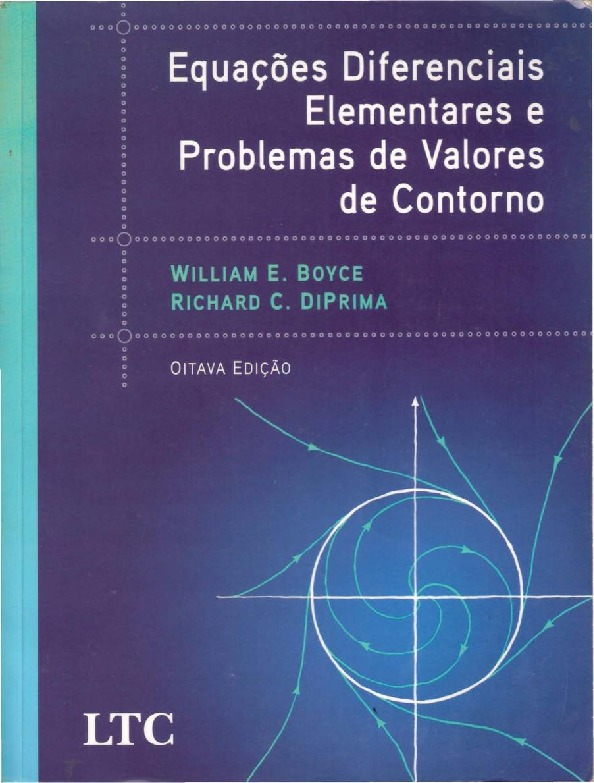
\includegraphics[width=0.8\linewidth]{figure/capa.jpg}    
    \end{flushright}
  \end{minipage}
  \vspace{0.25cm}
  \textcolor{mainColor}{\hrule}
  
  \begin{center}
    \vspace{0.5cm}
        \large{\textbf{Capítulo 1: }}
            \large{\textbf{Introdução}}
        \vspace{0.5cm}
  \end{center}
}


\begin{document}
\thispagestyle{empty}

\makeheader


\noindent Nos problemas de 1 a 6, desenha um campo de direções para a equação diferencial dada. Determine o comportamento de \(y\) quando \(t \rightarrow \infty\). Se esse comportamento depender do valor inicial de \(y\) quando \(t = 0\), descreva essa dependência.

\begin{enumerate}
    \item $y^\prime = 3 - 2y$
\end{enumerate}

\iniSol

Inicialmente, determinemos a solução de equilíbrio:

\begin{align*}
    y^\prime = 0 &\Rightarrow 3 - 2y = 0 \Rightarrow y = \dfrac{3}{2} = 1.50
\end{align*}

Como ilustra o campo de direções abaixo, todas as soluções tendem à solução de equilíbrio quando \(t\rightarrow \infty\).

\begin{figure}[H]
\centering
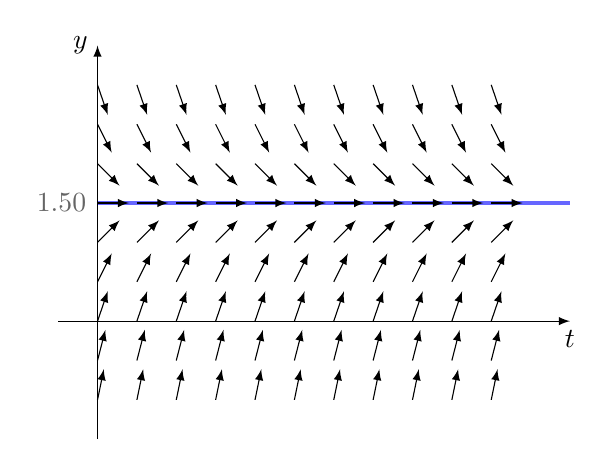
\begin{tikzpicture}
  \draw[-latex] (-0.50, 0)--(6.00, 0) node[below] {$t$};\draw[-latex] (0, -1.50)--(0, 3.50) node[left] {$y$}; \draw[ultra thick, opacity=0.6, blue] (6.00, 1.50)--(0.00, 1.50) node[left, black, fill=white] {$1.50$};\draw[-latex] (0.00, -1.00) -- (0.08 , -0.61);\draw[-latex] (0.00, -0.50) -- (0.10 , -0.11);\draw[-latex] (0.00, 0.00) -- (0.13 , 0.38);\draw[-latex] (0.00, 0.50) -- (0.18 , 0.86);\draw[-latex] (0.00, 1.00) -- (0.28 , 1.28);\draw[-latex] (0.00, 1.50) -- (0.40 , 1.50);\draw[-latex] (0.00, 2.00) -- (0.28 , 1.72);\draw[-latex] (0.00, 2.50) -- (0.18 , 2.14);\draw[-latex] (0.00, 3.00) -- (0.13 , 2.62);\draw[-latex] (0.50, -1.00) -- (0.58 , -0.61);\draw[-latex] (0.50, -0.50) -- (0.60 , -0.11);\draw[-latex] (0.50, 0.00) -- (0.63 , 0.38);\draw[-latex] (0.50, 0.50) -- (0.68 , 0.86);\draw[-latex] (0.50, 1.00) -- (0.78 , 1.28);\draw[-latex] (0.50, 1.50) -- (0.90 , 1.50);\draw[-latex] (0.50, 2.00) -- (0.78 , 1.72);\draw[-latex] (0.50, 2.50) -- (0.68 , 2.14);\draw[-latex] (0.50, 3.00) -- (0.63 , 2.62);\draw[-latex] (1.00, -1.00) -- (1.08 , -0.61);\draw[-latex] (1.00, -0.50) -- (1.10 , -0.11);\draw[-latex] (1.00, 0.00) -- (1.13 , 0.38);\draw[-latex] (1.00, 0.50) -- (1.18 , 0.86);\draw[-latex] (1.00, 1.00) -- (1.28 , 1.28);\draw[-latex] (1.00, 1.50) -- (1.40 , 1.50);\draw[-latex] (1.00, 2.00) -- (1.28 , 1.72);\draw[-latex] (1.00, 2.50) -- (1.18 , 2.14);\draw[-latex] (1.00, 3.00) -- (1.13 , 2.62);\draw[-latex] (1.50, -1.00) -- (1.58 , -0.61);\draw[-latex] (1.50, -0.50) -- (1.60 , -0.11);\draw[-latex] (1.50, 0.00) -- (1.63 , 0.38);\draw[-latex] (1.50, 0.50) -- (1.68 , 0.86);\draw[-latex] (1.50, 1.00) -- (1.78 , 1.28);\draw[-latex] (1.50, 1.50) -- (1.90 , 1.50);\draw[-latex] (1.50, 2.00) -- (1.78 , 1.72);\draw[-latex] (1.50, 2.50) -- (1.68 , 2.14);\draw[-latex] (1.50, 3.00) -- (1.63 , 2.62);\draw[-latex] (2.00, -1.00) -- (2.08 , -0.61);\draw[-latex] (2.00, -0.50) -- (2.10 , -0.11);\draw[-latex] (2.00, 0.00) -- (2.13 , 0.38);\draw[-latex] (2.00, 0.50) -- (2.18 , 0.86);\draw[-latex] (2.00, 1.00) -- (2.28 , 1.28);\draw[-latex] (2.00, 1.50) -- (2.40 , 1.50);\draw[-latex] (2.00, 2.00) -- (2.28 , 1.72);\draw[-latex] (2.00, 2.50) -- (2.18 , 2.14);\draw[-latex] (2.00, 3.00) -- (2.13 , 2.62);\draw[-latex] (2.50, -1.00) -- (2.58 , -0.61);\draw[-latex] (2.50, -0.50) -- (2.60 , -0.11);\draw[-latex] (2.50, 0.00) -- (2.63 , 0.38);\draw[-latex] (2.50, 0.50) -- (2.68 , 0.86);\draw[-latex] (2.50, 1.00) -- (2.78 , 1.28);\draw[-latex] (2.50, 1.50) -- (2.90 , 1.50);\draw[-latex] (2.50, 2.00) -- (2.78 , 1.72);\draw[-latex] (2.50, 2.50) -- (2.68 , 2.14);\draw[-latex] (2.50, 3.00) -- (2.63 , 2.62);\draw[-latex] (3.00, -1.00) -- (3.08 , -0.61);\draw[-latex] (3.00, -0.50) -- (3.10 , -0.11);\draw[-latex] (3.00, 0.00) -- (3.13 , 0.38);\draw[-latex] (3.00, 0.50) -- (3.18 , 0.86);\draw[-latex] (3.00, 1.00) -- (3.28 , 1.28);\draw[-latex] (3.00, 1.50) -- (3.40 , 1.50);\draw[-latex] (3.00, 2.00) -- (3.28 , 1.72);\draw[-latex] (3.00, 2.50) -- (3.18 , 2.14);\draw[-latex] (3.00, 3.00) -- (3.13 , 2.62);\draw[-latex] (3.50, -1.00) -- (3.58 , -0.61);\draw[-latex] (3.50, -0.50) -- (3.60 , -0.11);\draw[-latex] (3.50, 0.00) -- (3.63 , 0.38);\draw[-latex] (3.50, 0.50) -- (3.68 , 0.86);\draw[-latex] (3.50, 1.00) -- (3.78 , 1.28);\draw[-latex] (3.50, 1.50) -- (3.90 , 1.50);\draw[-latex] (3.50, 2.00) -- (3.78 , 1.72);\draw[-latex] (3.50, 2.50) -- (3.68 , 2.14);\draw[-latex] (3.50, 3.00) -- (3.63 , 2.62);\draw[-latex] (4.00, -1.00) -- (4.08 , -0.61);\draw[-latex] (4.00, -0.50) -- (4.10 , -0.11);\draw[-latex] (4.00, 0.00) -- (4.13 , 0.38);\draw[-latex] (4.00, 0.50) -- (4.18 , 0.86);\draw[-latex] (4.00, 1.00) -- (4.28 , 1.28);\draw[-latex] (4.00, 1.50) -- (4.40 , 1.50);\draw[-latex] (4.00, 2.00) -- (4.28 , 1.72);\draw[-latex] (4.00, 2.50) -- (4.18 , 2.14);\draw[-latex] (4.00, 3.00) -- (4.13 , 2.62);\draw[-latex] (4.50, -1.00) -- (4.58 , -0.61);\draw[-latex] (4.50, -0.50) -- (4.60 , -0.11);\draw[-latex] (4.50, 0.00) -- (4.63 , 0.38);\draw[-latex] (4.50, 0.50) -- (4.68 , 0.86);\draw[-latex] (4.50, 1.00) -- (4.78 , 1.28);\draw[-latex] (4.50, 1.50) -- (4.90 , 1.50);\draw[-latex] (4.50, 2.00) -- (4.78 , 1.72);\draw[-latex] (4.50, 2.50) -- (4.68 , 2.14);\draw[-latex] (4.50, 3.00) -- (4.63 , 2.62);\draw[-latex] (5.00, -1.00) -- (5.08 , -0.61);\draw[-latex] (5.00, -0.50) -- (5.10 , -0.11);\draw[-latex] (5.00, 0.00) -- (5.13 , 0.38);\draw[-latex] (5.00, 0.50) -- (5.18 , 0.86);\draw[-latex] (5.00, 1.00) -- (5.28 , 1.28);\draw[-latex] (5.00, 1.50) -- (5.40 , 1.50);\draw[-latex] (5.00, 2.00) -- (5.28 , 1.72);\draw[-latex] (5.00, 2.50) -- (5.18 , 2.14);\draw[-latex] (5.00, 3.00) -- (5.13 , 2.62);
\end{tikzpicture}
\end{figure}

\fimSol

\begin{enumerate}[resume]
    \item $y^\prime = 2y-3$
\end{enumerate}

\iniSol

Inicialmente, determinemos a solução de equilíbrio:

\begin{align*}
    y^\prime = 0 &\Rightarrow 2y - 3 = 0 \Rightarrow y = \dfrac{3}{2} = 1.50
\end{align*}

Como ilustra o campo de direções abaixo, todas as soluções afastam-se solução de equilíbrio quando \(t\rightarrow \infty\).

\begin{figure}[H]
\centering
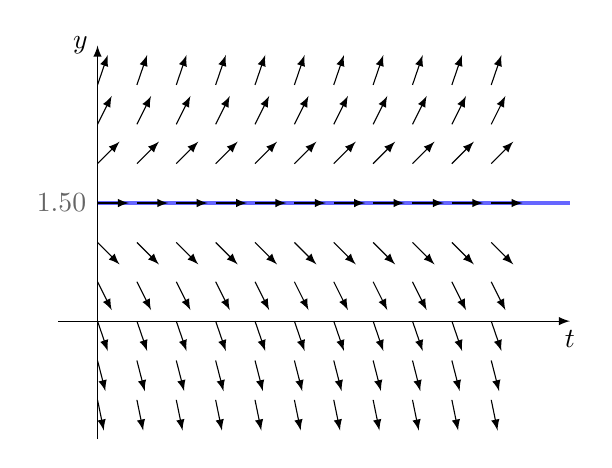
\begin{tikzpicture}
  \draw[-latex] (-0.50, 0)--(6.00, 0) node[below] {$t$};\draw[-latex] (0, -1.50)--(0, 3.50) node[left] {$y$}; \draw[ultra thick, opacity=0.6, blue] (6.00, 1.50)--(0.00, 1.50) node[left, black, fill=white] {$1.50$};\draw[-latex] (0.00, -1.00) -- (0.08 , -1.39);\draw[-latex] (0.00, -0.50) -- (0.10 , -0.89);\draw[-latex] (0.00, 0.00) -- (0.13 , -0.38);\draw[-latex] (0.00, 0.50) -- (0.18 , 0.14);\draw[-latex] (0.00, 1.00) -- (0.28 , 0.72);\draw[-latex] (0.00, 1.50) -- (0.40 , 1.50);\draw[-latex] (0.00, 2.00) -- (0.28 , 2.28);\draw[-latex] (0.00, 2.50) -- (0.18 , 2.86);\draw[-latex] (0.00, 3.00) -- (0.13 , 3.38);\draw[-latex] (0.50, -1.00) -- (0.58 , -1.39);\draw[-latex] (0.50, -0.50) -- (0.60 , -0.89);\draw[-latex] (0.50, 0.00) -- (0.63 , -0.38);\draw[-latex] (0.50, 0.50) -- (0.68 , 0.14);\draw[-latex] (0.50, 1.00) -- (0.78 , 0.72);\draw[-latex] (0.50, 1.50) -- (0.90 , 1.50);\draw[-latex] (0.50, 2.00) -- (0.78 , 2.28);\draw[-latex] (0.50, 2.50) -- (0.68 , 2.86);\draw[-latex] (0.50, 3.00) -- (0.63 , 3.38);\draw[-latex] (1.00, -1.00) -- (1.08 , -1.39);\draw[-latex] (1.00, -0.50) -- (1.10 , -0.89);\draw[-latex] (1.00, 0.00) -- (1.13 , -0.38);\draw[-latex] (1.00, 0.50) -- (1.18 , 0.14);\draw[-latex] (1.00, 1.00) -- (1.28 , 0.72);\draw[-latex] (1.00, 1.50) -- (1.40 , 1.50);\draw[-latex] (1.00, 2.00) -- (1.28 , 2.28);\draw[-latex] (1.00, 2.50) -- (1.18 , 2.86);\draw[-latex] (1.00, 3.00) -- (1.13 , 3.38);\draw[-latex] (1.50, -1.00) -- (1.58 , -1.39);\draw[-latex] (1.50, -0.50) -- (1.60 , -0.89);\draw[-latex] (1.50, 0.00) -- (1.63 , -0.38);\draw[-latex] (1.50, 0.50) -- (1.68 , 0.14);\draw[-latex] (1.50, 1.00) -- (1.78 , 0.72);\draw[-latex] (1.50, 1.50) -- (1.90 , 1.50);\draw[-latex] (1.50, 2.00) -- (1.78 , 2.28);\draw[-latex] (1.50, 2.50) -- (1.68 , 2.86);\draw[-latex] (1.50, 3.00) -- (1.63 , 3.38);\draw[-latex] (2.00, -1.00) -- (2.08 , -1.39);\draw[-latex] (2.00, -0.50) -- (2.10 , -0.89);\draw[-latex] (2.00, 0.00) -- (2.13 , -0.38);\draw[-latex] (2.00, 0.50) -- (2.18 , 0.14);\draw[-latex] (2.00, 1.00) -- (2.28 , 0.72);\draw[-latex] (2.00, 1.50) -- (2.40 , 1.50);\draw[-latex] (2.00, 2.00) -- (2.28 , 2.28);\draw[-latex] (2.00, 2.50) -- (2.18 , 2.86);\draw[-latex] (2.00, 3.00) -- (2.13 , 3.38);\draw[-latex] (2.50, -1.00) -- (2.58 , -1.39);\draw[-latex] (2.50, -0.50) -- (2.60 , -0.89);\draw[-latex] (2.50, 0.00) -- (2.63 , -0.38);\draw[-latex] (2.50, 0.50) -- (2.68 , 0.14);\draw[-latex] (2.50, 1.00) -- (2.78 , 0.72);\draw[-latex] (2.50, 1.50) -- (2.90 , 1.50);\draw[-latex] (2.50, 2.00) -- (2.78 , 2.28);\draw[-latex] (2.50, 2.50) -- (2.68 , 2.86);\draw[-latex] (2.50, 3.00) -- (2.63 , 3.38);\draw[-latex] (3.00, -1.00) -- (3.08 , -1.39);\draw[-latex] (3.00, -0.50) -- (3.10 , -0.89);\draw[-latex] (3.00, 0.00) -- (3.13 , -0.38);\draw[-latex] (3.00, 0.50) -- (3.18 , 0.14);\draw[-latex] (3.00, 1.00) -- (3.28 , 0.72);\draw[-latex] (3.00, 1.50) -- (3.40 , 1.50);\draw[-latex] (3.00, 2.00) -- (3.28 , 2.28);\draw[-latex] (3.00, 2.50) -- (3.18 , 2.86);\draw[-latex] (3.00, 3.00) -- (3.13 , 3.38);\draw[-latex] (3.50, -1.00) -- (3.58 , -1.39);\draw[-latex] (3.50, -0.50) -- (3.60 , -0.89);\draw[-latex] (3.50, 0.00) -- (3.63 , -0.38);\draw[-latex] (3.50, 0.50) -- (3.68 , 0.14);\draw[-latex] (3.50, 1.00) -- (3.78 , 0.72);\draw[-latex] (3.50, 1.50) -- (3.90 , 1.50);\draw[-latex] (3.50, 2.00) -- (3.78 , 2.28);\draw[-latex] (3.50, 2.50) -- (3.68 , 2.86);\draw[-latex] (3.50, 3.00) -- (3.63 , 3.38);\draw[-latex] (4.00, -1.00) -- (4.08 , -1.39);\draw[-latex] (4.00, -0.50) -- (4.10 , -0.89);\draw[-latex] (4.00, 0.00) -- (4.13 , -0.38);\draw[-latex] (4.00, 0.50) -- (4.18 , 0.14);\draw[-latex] (4.00, 1.00) -- (4.28 , 0.72);\draw[-latex] (4.00, 1.50) -- (4.40 , 1.50);\draw[-latex] (4.00, 2.00) -- (4.28 , 2.28);\draw[-latex] (4.00, 2.50) -- (4.18 , 2.86);\draw[-latex] (4.00, 3.00) -- (4.13 , 3.38);\draw[-latex] (4.50, -1.00) -- (4.58 , -1.39);\draw[-latex] (4.50, -0.50) -- (4.60 , -0.89);\draw[-latex] (4.50, 0.00) -- (4.63 , -0.38);\draw[-latex] (4.50, 0.50) -- (4.68 , 0.14);\draw[-latex] (4.50, 1.00) -- (4.78 , 0.72);\draw[-latex] (4.50, 1.50) -- (4.90 , 1.50);\draw[-latex] (4.50, 2.00) -- (4.78 , 2.28);\draw[-latex] (4.50, 2.50) -- (4.68 , 2.86);\draw[-latex] (4.50, 3.00) -- (4.63 , 3.38);\draw[-latex] (5.00, -1.00) -- (5.08 , -1.39);\draw[-latex] (5.00, -0.50) -- (5.10 , -0.89);\draw[-latex] (5.00, 0.00) -- (5.13 , -0.38);\draw[-latex] (5.00, 0.50) -- (5.18 , 0.14);\draw[-latex] (5.00, 1.00) -- (5.28 , 0.72);\draw[-latex] (5.00, 1.50) -- (5.40 , 1.50);\draw[-latex] (5.00, 2.00) -- (5.28 , 2.28);\draw[-latex] (5.00, 2.50) -- (5.18 , 2.86);\draw[-latex] (5.00, 3.00) -- (5.13 , 3.38);
\end{tikzpicture}
\end{figure}

\fimSol

\begin{enumerate}[resume]
    \item $y^\prime = 3+2y$
\end{enumerate}

\iniSol

Inicialmente, determinemos a solução de equilíbrio:

\begin{align*}
    y^\prime = 0 &\Rightarrow 3+2y = 0 \Rightarrow y = -\dfrac{3}{2} = -1.50
\end{align*}

Como ilustra o campo de direções abaixo, todas as soluções afastam-se solução de equilíbrio quando \(t\rightarrow \infty\).

\begin{figure}[H]
\centering
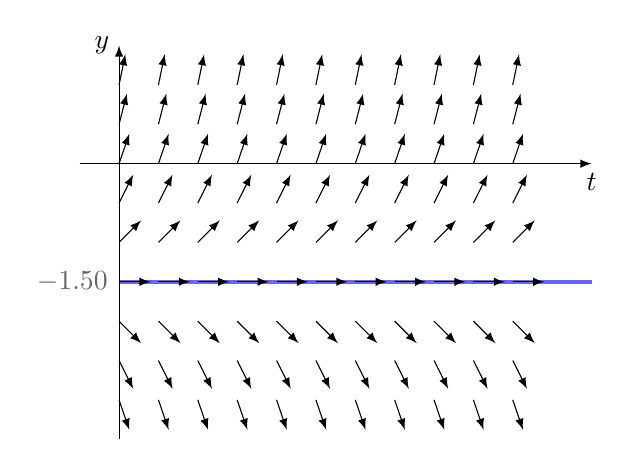
\begin{tikzpicture}
  \draw[-latex] (-0.50, 0)--(6.00, 0) node[below] {$t$};\draw[-latex] (0, -3.50)--(0, 1.50) node[left] {$y$}; \draw[ultra thick, opacity=0.6, blue] (6.00, -1.50)--(0.00, -1.50) node[left, black, fill=white] {$-1.50$};\draw[-latex] (0.00, -3.00) -- (0.13 , -3.38);\draw[-latex] (0.00, -2.50) -- (0.18 , -2.86);\draw[-latex] (0.00, -2.00) -- (0.28 , -2.28);\draw[-latex] (0.00, -1.50) -- (0.40 , -1.50);\draw[-latex] (0.00, -1.00) -- (0.28 , -0.72);\draw[-latex] (0.00, -0.50) -- (0.18 , -0.14);\draw[-latex] (0.00, 0.00) -- (0.13 , 0.38);\draw[-latex] (0.00, 0.50) -- (0.10 , 0.89);\draw[-latex] (0.00, 1.00) -- (0.08 , 1.39);\draw[-latex] (0.50, -3.00) -- (0.63 , -3.38);\draw[-latex] (0.50, -2.50) -- (0.68 , -2.86);\draw[-latex] (0.50, -2.00) -- (0.78 , -2.28);\draw[-latex] (0.50, -1.50) -- (0.90 , -1.50);\draw[-latex] (0.50, -1.00) -- (0.78 , -0.72);\draw[-latex] (0.50, -0.50) -- (0.68 , -0.14);\draw[-latex] (0.50, 0.00) -- (0.63 , 0.38);\draw[-latex] (0.50, 0.50) -- (0.60 , 0.89);\draw[-latex] (0.50, 1.00) -- (0.58 , 1.39);\draw[-latex] (1.00, -3.00) -- (1.13 , -3.38);\draw[-latex] (1.00, -2.50) -- (1.18 , -2.86);\draw[-latex] (1.00, -2.00) -- (1.28 , -2.28);\draw[-latex] (1.00, -1.50) -- (1.40 , -1.50);\draw[-latex] (1.00, -1.00) -- (1.28 , -0.72);\draw[-latex] (1.00, -0.50) -- (1.18 , -0.14);\draw[-latex] (1.00, 0.00) -- (1.13 , 0.38);\draw[-latex] (1.00, 0.50) -- (1.10 , 0.89);\draw[-latex] (1.00, 1.00) -- (1.08 , 1.39);\draw[-latex] (1.50, -3.00) -- (1.63 , -3.38);\draw[-latex] (1.50, -2.50) -- (1.68 , -2.86);\draw[-latex] (1.50, -2.00) -- (1.78 , -2.28);\draw[-latex] (1.50, -1.50) -- (1.90 , -1.50);\draw[-latex] (1.50, -1.00) -- (1.78 , -0.72);\draw[-latex] (1.50, -0.50) -- (1.68 , -0.14);\draw[-latex] (1.50, 0.00) -- (1.63 , 0.38);\draw[-latex] (1.50, 0.50) -- (1.60 , 0.89);\draw[-latex] (1.50, 1.00) -- (1.58 , 1.39);\draw[-latex] (2.00, -3.00) -- (2.13 , -3.38);\draw[-latex] (2.00, -2.50) -- (2.18 , -2.86);\draw[-latex] (2.00, -2.00) -- (2.28 , -2.28);\draw[-latex] (2.00, -1.50) -- (2.40 , -1.50);\draw[-latex] (2.00, -1.00) -- (2.28 , -0.72);\draw[-latex] (2.00, -0.50) -- (2.18 , -0.14);\draw[-latex] (2.00, 0.00) -- (2.13 , 0.38);\draw[-latex] (2.00, 0.50) -- (2.10 , 0.89);\draw[-latex] (2.00, 1.00) -- (2.08 , 1.39);\draw[-latex] (2.50, -3.00) -- (2.63 , -3.38);\draw[-latex] (2.50, -2.50) -- (2.68 , -2.86);\draw[-latex] (2.50, -2.00) -- (2.78 , -2.28);\draw[-latex] (2.50, -1.50) -- (2.90 , -1.50);\draw[-latex] (2.50, -1.00) -- (2.78 , -0.72);\draw[-latex] (2.50, -0.50) -- (2.68 , -0.14);\draw[-latex] (2.50, 0.00) -- (2.63 , 0.38);\draw[-latex] (2.50, 0.50) -- (2.60 , 0.89);\draw[-latex] (2.50, 1.00) -- (2.58 , 1.39);\draw[-latex] (3.00, -3.00) -- (3.13 , -3.38);\draw[-latex] (3.00, -2.50) -- (3.18 , -2.86);\draw[-latex] (3.00, -2.00) -- (3.28 , -2.28);\draw[-latex] (3.00, -1.50) -- (3.40 , -1.50);\draw[-latex] (3.00, -1.00) -- (3.28 , -0.72);\draw[-latex] (3.00, -0.50) -- (3.18 , -0.14);\draw[-latex] (3.00, 0.00) -- (3.13 , 0.38);\draw[-latex] (3.00, 0.50) -- (3.10 , 0.89);\draw[-latex] (3.00, 1.00) -- (3.08 , 1.39);\draw[-latex] (3.50, -3.00) -- (3.63 , -3.38);\draw[-latex] (3.50, -2.50) -- (3.68 , -2.86);\draw[-latex] (3.50, -2.00) -- (3.78 , -2.28);\draw[-latex] (3.50, -1.50) -- (3.90 , -1.50);\draw[-latex] (3.50, -1.00) -- (3.78 , -0.72);\draw[-latex] (3.50, -0.50) -- (3.68 , -0.14);\draw[-latex] (3.50, 0.00) -- (3.63 , 0.38);\draw[-latex] (3.50, 0.50) -- (3.60 , 0.89);\draw[-latex] (3.50, 1.00) -- (3.58 , 1.39);\draw[-latex] (4.00, -3.00) -- (4.13 , -3.38);\draw[-latex] (4.00, -2.50) -- (4.18 , -2.86);\draw[-latex] (4.00, -2.00) -- (4.28 , -2.28);\draw[-latex] (4.00, -1.50) -- (4.40 , -1.50);\draw[-latex] (4.00, -1.00) -- (4.28 , -0.72);\draw[-latex] (4.00, -0.50) -- (4.18 , -0.14);\draw[-latex] (4.00, 0.00) -- (4.13 , 0.38);\draw[-latex] (4.00, 0.50) -- (4.10 , 0.89);\draw[-latex] (4.00, 1.00) -- (4.08 , 1.39);\draw[-latex] (4.50, -3.00) -- (4.63 , -3.38);\draw[-latex] (4.50, -2.50) -- (4.68 , -2.86);\draw[-latex] (4.50, -2.00) -- (4.78 , -2.28);\draw[-latex] (4.50, -1.50) -- (4.90 , -1.50);\draw[-latex] (4.50, -1.00) -- (4.78 , -0.72);\draw[-latex] (4.50, -0.50) -- (4.68 , -0.14);\draw[-latex] (4.50, 0.00) -- (4.63 , 0.38);\draw[-latex] (4.50, 0.50) -- (4.60 , 0.89);\draw[-latex] (4.50, 1.00) -- (4.58 , 1.39);\draw[-latex] (5.00, -3.00) -- (5.13 , -3.38);\draw[-latex] (5.00, -2.50) -- (5.18 , -2.86);\draw[-latex] (5.00, -2.00) -- (5.28 , -2.28);\draw[-latex] (5.00, -1.50) -- (5.40 , -1.50);\draw[-latex] (5.00, -1.00) -- (5.28 , -0.72);\draw[-latex] (5.00, -0.50) -- (5.18 , -0.14);\draw[-latex] (5.00, 0.00) -- (5.13 , 0.38);\draw[-latex] (5.00, 0.50) -- (5.10 , 0.89);\draw[-latex] (5.00, 1.00) -- (5.08 , 1.39);
\end{tikzpicture}
\end{figure}

\fimSol

\begin{enumerate}[resume]
    \item $y^\prime = -1-2y$
\end{enumerate}

\iniSol

Inicialmente, determinemos a solução de equilíbrio:

\begin{align*}
    y^\prime = 0 &\Rightarrow -1-2y = 0 \Rightarrow y = -\dfrac{1}{2} = -0.50
\end{align*}

Como ilustra o campo de direções abaixo, todas as soluções tendem à solução de equilíbrio quando \(t\rightarrow \infty\).

\begin{figure}[H]
\centering
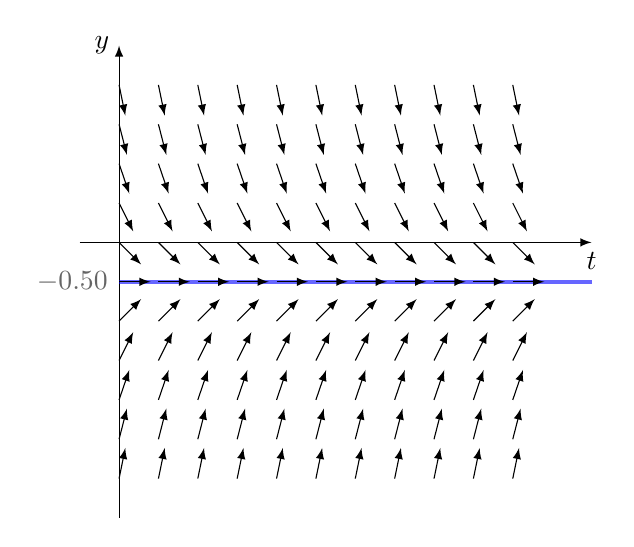
\begin{tikzpicture}
  \draw[-latex] (-0.50, 0)--(6.00, 0) node[below] {$t$};\draw[-latex] (0, -3.50)--(0, 2.50) node[left] {$y$}; \draw[ultra thick, opacity=0.6, blue] (6.00, -0.50)--(0.00, -0.50) node[left, black, fill=white] {$-0.50$};\draw[-latex] (0.00, -3.00) -- (0.08 , -2.61);\draw[-latex] (0.00, -2.50) -- (0.10 , -2.11);\draw[-latex] (0.00, -2.00) -- (0.13 , -1.62);\draw[-latex] (0.00, -1.50) -- (0.18 , -1.14);\draw[-latex] (0.00, -1.00) -- (0.28 , -0.72);\draw[-latex] (0.00, -0.50) -- (0.40 , -0.50);\draw[-latex] (0.00, 0.00) -- (0.28 , -0.28);\draw[-latex] (0.00, 0.50) -- (0.18 , 0.14);\draw[-latex] (0.00, 1.00) -- (0.13 , 0.62);\draw[-latex] (0.00, 1.50) -- (0.10 , 1.11);\draw[-latex] (0.00, 2.00) -- (0.08 , 1.61);\draw[-latex] (0.50, -3.00) -- (0.58 , -2.61);\draw[-latex] (0.50, -2.50) -- (0.60 , -2.11);\draw[-latex] (0.50, -2.00) -- (0.63 , -1.62);\draw[-latex] (0.50, -1.50) -- (0.68 , -1.14);\draw[-latex] (0.50, -1.00) -- (0.78 , -0.72);\draw[-latex] (0.50, -0.50) -- (0.90 , -0.50);\draw[-latex] (0.50, 0.00) -- (0.78 , -0.28);\draw[-latex] (0.50, 0.50) -- (0.68 , 0.14);\draw[-latex] (0.50, 1.00) -- (0.63 , 0.62);\draw[-latex] (0.50, 1.50) -- (0.60 , 1.11);\draw[-latex] (0.50, 2.00) -- (0.58 , 1.61);\draw[-latex] (1.00, -3.00) -- (1.08 , -2.61);\draw[-latex] (1.00, -2.50) -- (1.10 , -2.11);\draw[-latex] (1.00, -2.00) -- (1.13 , -1.62);\draw[-latex] (1.00, -1.50) -- (1.18 , -1.14);\draw[-latex] (1.00, -1.00) -- (1.28 , -0.72);\draw[-latex] (1.00, -0.50) -- (1.40 , -0.50);\draw[-latex] (1.00, 0.00) -- (1.28 , -0.28);\draw[-latex] (1.00, 0.50) -- (1.18 , 0.14);\draw[-latex] (1.00, 1.00) -- (1.13 , 0.62);\draw[-latex] (1.00, 1.50) -- (1.10 , 1.11);\draw[-latex] (1.00, 2.00) -- (1.08 , 1.61);\draw[-latex] (1.50, -3.00) -- (1.58 , -2.61);\draw[-latex] (1.50, -2.50) -- (1.60 , -2.11);\draw[-latex] (1.50, -2.00) -- (1.63 , -1.62);\draw[-latex] (1.50, -1.50) -- (1.68 , -1.14);\draw[-latex] (1.50, -1.00) -- (1.78 , -0.72);\draw[-latex] (1.50, -0.50) -- (1.90 , -0.50);\draw[-latex] (1.50, 0.00) -- (1.78 , -0.28);\draw[-latex] (1.50, 0.50) -- (1.68 , 0.14);\draw[-latex] (1.50, 1.00) -- (1.63 , 0.62);\draw[-latex] (1.50, 1.50) -- (1.60 , 1.11);\draw[-latex] (1.50, 2.00) -- (1.58 , 1.61);\draw[-latex] (2.00, -3.00) -- (2.08 , -2.61);\draw[-latex] (2.00, -2.50) -- (2.10 , -2.11);\draw[-latex] (2.00, -2.00) -- (2.13 , -1.62);\draw[-latex] (2.00, -1.50) -- (2.18 , -1.14);\draw[-latex] (2.00, -1.00) -- (2.28 , -0.72);\draw[-latex] (2.00, -0.50) -- (2.40 , -0.50);\draw[-latex] (2.00, 0.00) -- (2.28 , -0.28);\draw[-latex] (2.00, 0.50) -- (2.18 , 0.14);\draw[-latex] (2.00, 1.00) -- (2.13 , 0.62);\draw[-latex] (2.00, 1.50) -- (2.10 , 1.11);\draw[-latex] (2.00, 2.00) -- (2.08 , 1.61);\draw[-latex] (2.50, -3.00) -- (2.58 , -2.61);\draw[-latex] (2.50, -2.50) -- (2.60 , -2.11);\draw[-latex] (2.50, -2.00) -- (2.63 , -1.62);\draw[-latex] (2.50, -1.50) -- (2.68 , -1.14);\draw[-latex] (2.50, -1.00) -- (2.78 , -0.72);\draw[-latex] (2.50, -0.50) -- (2.90 , -0.50);\draw[-latex] (2.50, 0.00) -- (2.78 , -0.28);\draw[-latex] (2.50, 0.50) -- (2.68 , 0.14);\draw[-latex] (2.50, 1.00) -- (2.63 , 0.62);\draw[-latex] (2.50, 1.50) -- (2.60 , 1.11);\draw[-latex] (2.50, 2.00) -- (2.58 , 1.61);\draw[-latex] (3.00, -3.00) -- (3.08 , -2.61);\draw[-latex] (3.00, -2.50) -- (3.10 , -2.11);\draw[-latex] (3.00, -2.00) -- (3.13 , -1.62);\draw[-latex] (3.00, -1.50) -- (3.18 , -1.14);\draw[-latex] (3.00, -1.00) -- (3.28 , -0.72);\draw[-latex] (3.00, -0.50) -- (3.40 , -0.50);\draw[-latex] (3.00, 0.00) -- (3.28 , -0.28);\draw[-latex] (3.00, 0.50) -- (3.18 , 0.14);\draw[-latex] (3.00, 1.00) -- (3.13 , 0.62);\draw[-latex] (3.00, 1.50) -- (3.10 , 1.11);\draw[-latex] (3.00, 2.00) -- (3.08 , 1.61);\draw[-latex] (3.50, -3.00) -- (3.58 , -2.61);\draw[-latex] (3.50, -2.50) -- (3.60 , -2.11);\draw[-latex] (3.50, -2.00) -- (3.63 , -1.62);\draw[-latex] (3.50, -1.50) -- (3.68 , -1.14);\draw[-latex] (3.50, -1.00) -- (3.78 , -0.72);\draw[-latex] (3.50, -0.50) -- (3.90 , -0.50);\draw[-latex] (3.50, 0.00) -- (3.78 , -0.28);\draw[-latex] (3.50, 0.50) -- (3.68 , 0.14);\draw[-latex] (3.50, 1.00) -- (3.63 , 0.62);\draw[-latex] (3.50, 1.50) -- (3.60 , 1.11);\draw[-latex] (3.50, 2.00) -- (3.58 , 1.61);\draw[-latex] (4.00, -3.00) -- (4.08 , -2.61);\draw[-latex] (4.00, -2.50) -- (4.10 , -2.11);\draw[-latex] (4.00, -2.00) -- (4.13 , -1.62);\draw[-latex] (4.00, -1.50) -- (4.18 , -1.14);\draw[-latex] (4.00, -1.00) -- (4.28 , -0.72);\draw[-latex] (4.00, -0.50) -- (4.40 , -0.50);\draw[-latex] (4.00, 0.00) -- (4.28 , -0.28);\draw[-latex] (4.00, 0.50) -- (4.18 , 0.14);\draw[-latex] (4.00, 1.00) -- (4.13 , 0.62);\draw[-latex] (4.00, 1.50) -- (4.10 , 1.11);\draw[-latex] (4.00, 2.00) -- (4.08 , 1.61);\draw[-latex] (4.50, -3.00) -- (4.58 , -2.61);\draw[-latex] (4.50, -2.50) -- (4.60 , -2.11);\draw[-latex] (4.50, -2.00) -- (4.63 , -1.62);\draw[-latex] (4.50, -1.50) -- (4.68 , -1.14);\draw[-latex] (4.50, -1.00) -- (4.78 , -0.72);\draw[-latex] (4.50, -0.50) -- (4.90 , -0.50);\draw[-latex] (4.50, 0.00) -- (4.78 , -0.28);\draw[-latex] (4.50, 0.50) -- (4.68 , 0.14);\draw[-latex] (4.50, 1.00) -- (4.63 , 0.62);\draw[-latex] (4.50, 1.50) -- (4.60 , 1.11);\draw[-latex] (4.50, 2.00) -- (4.58 , 1.61);\draw[-latex] (5.00, -3.00) -- (5.08 , -2.61);\draw[-latex] (5.00, -2.50) -- (5.10 , -2.11);\draw[-latex] (5.00, -2.00) -- (5.13 , -1.62);\draw[-latex] (5.00, -1.50) -- (5.18 , -1.14);\draw[-latex] (5.00, -1.00) -- (5.28 , -0.72);\draw[-latex] (5.00, -0.50) -- (5.40 , -0.50);\draw[-latex] (5.00, 0.00) -- (5.28 , -0.28);\draw[-latex] (5.00, 0.50) -- (5.18 , 0.14);\draw[-latex] (5.00, 1.00) -- (5.13 , 0.62);\draw[-latex] (5.00, 1.50) -- (5.10 , 1.11);\draw[-latex] (5.00, 2.00) -- (5.08 , 1.61);
\end{tikzpicture}
\end{figure}

\fimSol

\begin{enumerate}[resume]
    \item $y^\prime = 1+2y$
\end{enumerate}

\iniSol

Inicialmente, determinemos a solução de equilíbrio:

\begin{align*}
    y^\prime = 0 &\Rightarrow 1+2y = 0 \Rightarrow y = -\dfrac{1}{2} = -0.50
\end{align*}

Como ilustra o campo de direções abaixo, todas as soluções afastam-se da solução de equilíbrio quando \(t\rightarrow \infty\).

\begin{figure}[H]
\centering
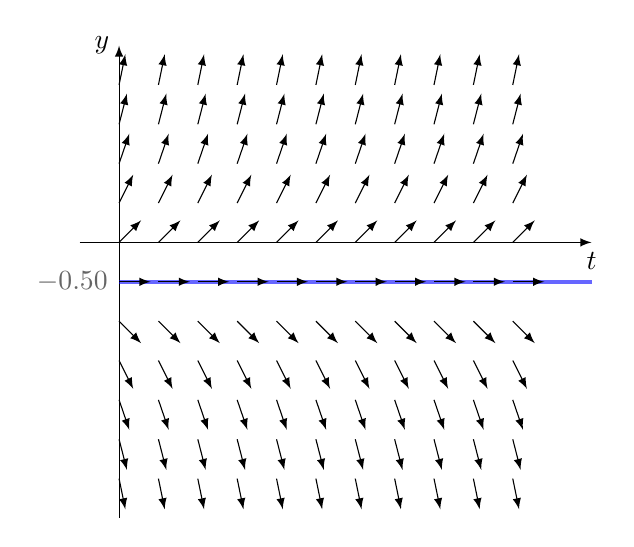
\begin{tikzpicture}
  \draw[-latex] (-0.50, 0)--(6.00, 0) node[below] {$t$};\draw[-latex] (0, -3.50)--(0, 2.50) node[left] {$y$}; \draw[ultra thick, opacity=0.6, blue] (6.00, -0.50)--(0.00, -0.50) node[left, black, fill=white] {$-0.50$};\draw[-latex] (0.00, -3.00) -- (0.08 , -3.39);\draw[-latex] (0.00, -2.50) -- (0.10 , -2.89);\draw[-latex] (0.00, -2.00) -- (0.13 , -2.38);\draw[-latex] (0.00, -1.50) -- (0.18 , -1.86);\draw[-latex] (0.00, -1.00) -- (0.28 , -1.28);\draw[-latex] (0.00, -0.50) -- (0.40 , -0.50);\draw[-latex] (0.00, 0.00) -- (0.28 , 0.28);\draw[-latex] (0.00, 0.50) -- (0.18 , 0.86);\draw[-latex] (0.00, 1.00) -- (0.13 , 1.38);\draw[-latex] (0.00, 1.50) -- (0.10 , 1.89);\draw[-latex] (0.00, 2.00) -- (0.08 , 2.39);\draw[-latex] (0.50, -3.00) -- (0.58 , -3.39);\draw[-latex] (0.50, -2.50) -- (0.60 , -2.89);\draw[-latex] (0.50, -2.00) -- (0.63 , -2.38);\draw[-latex] (0.50, -1.50) -- (0.68 , -1.86);\draw[-latex] (0.50, -1.00) -- (0.78 , -1.28);\draw[-latex] (0.50, -0.50) -- (0.90 , -0.50);\draw[-latex] (0.50, 0.00) -- (0.78 , 0.28);\draw[-latex] (0.50, 0.50) -- (0.68 , 0.86);\draw[-latex] (0.50, 1.00) -- (0.63 , 1.38);\draw[-latex] (0.50, 1.50) -- (0.60 , 1.89);\draw[-latex] (0.50, 2.00) -- (0.58 , 2.39);\draw[-latex] (1.00, -3.00) -- (1.08 , -3.39);\draw[-latex] (1.00, -2.50) -- (1.10 , -2.89);\draw[-latex] (1.00, -2.00) -- (1.13 , -2.38);\draw[-latex] (1.00, -1.50) -- (1.18 , -1.86);\draw[-latex] (1.00, -1.00) -- (1.28 , -1.28);\draw[-latex] (1.00, -0.50) -- (1.40 , -0.50);\draw[-latex] (1.00, 0.00) -- (1.28 , 0.28);\draw[-latex] (1.00, 0.50) -- (1.18 , 0.86);\draw[-latex] (1.00, 1.00) -- (1.13 , 1.38);\draw[-latex] (1.00, 1.50) -- (1.10 , 1.89);\draw[-latex] (1.00, 2.00) -- (1.08 , 2.39);\draw[-latex] (1.50, -3.00) -- (1.58 , -3.39);\draw[-latex] (1.50, -2.50) -- (1.60 , -2.89);\draw[-latex] (1.50, -2.00) -- (1.63 , -2.38);\draw[-latex] (1.50, -1.50) -- (1.68 , -1.86);\draw[-latex] (1.50, -1.00) -- (1.78 , -1.28);\draw[-latex] (1.50, -0.50) -- (1.90 , -0.50);\draw[-latex] (1.50, 0.00) -- (1.78 , 0.28);\draw[-latex] (1.50, 0.50) -- (1.68 , 0.86);\draw[-latex] (1.50, 1.00) -- (1.63 , 1.38);\draw[-latex] (1.50, 1.50) -- (1.60 , 1.89);\draw[-latex] (1.50, 2.00) -- (1.58 , 2.39);\draw[-latex] (2.00, -3.00) -- (2.08 , -3.39);\draw[-latex] (2.00, -2.50) -- (2.10 , -2.89);\draw[-latex] (2.00, -2.00) -- (2.13 , -2.38);\draw[-latex] (2.00, -1.50) -- (2.18 , -1.86);\draw[-latex] (2.00, -1.00) -- (2.28 , -1.28);\draw[-latex] (2.00, -0.50) -- (2.40 , -0.50);\draw[-latex] (2.00, 0.00) -- (2.28 , 0.28);\draw[-latex] (2.00, 0.50) -- (2.18 , 0.86);\draw[-latex] (2.00, 1.00) -- (2.13 , 1.38);\draw[-latex] (2.00, 1.50) -- (2.10 , 1.89);\draw[-latex] (2.00, 2.00) -- (2.08 , 2.39);\draw[-latex] (2.50, -3.00) -- (2.58 , -3.39);\draw[-latex] (2.50, -2.50) -- (2.60 , -2.89);\draw[-latex] (2.50, -2.00) -- (2.63 , -2.38);\draw[-latex] (2.50, -1.50) -- (2.68 , -1.86);\draw[-latex] (2.50, -1.00) -- (2.78 , -1.28);\draw[-latex] (2.50, -0.50) -- (2.90 , -0.50);\draw[-latex] (2.50, 0.00) -- (2.78 , 0.28);\draw[-latex] (2.50, 0.50) -- (2.68 , 0.86);\draw[-latex] (2.50, 1.00) -- (2.63 , 1.38);\draw[-latex] (2.50, 1.50) -- (2.60 , 1.89);\draw[-latex] (2.50, 2.00) -- (2.58 , 2.39);\draw[-latex] (3.00, -3.00) -- (3.08 , -3.39);\draw[-latex] (3.00, -2.50) -- (3.10 , -2.89);\draw[-latex] (3.00, -2.00) -- (3.13 , -2.38);\draw[-latex] (3.00, -1.50) -- (3.18 , -1.86);\draw[-latex] (3.00, -1.00) -- (3.28 , -1.28);\draw[-latex] (3.00, -0.50) -- (3.40 , -0.50);\draw[-latex] (3.00, 0.00) -- (3.28 , 0.28);\draw[-latex] (3.00, 0.50) -- (3.18 , 0.86);\draw[-latex] (3.00, 1.00) -- (3.13 , 1.38);\draw[-latex] (3.00, 1.50) -- (3.10 , 1.89);\draw[-latex] (3.00, 2.00) -- (3.08 , 2.39);\draw[-latex] (3.50, -3.00) -- (3.58 , -3.39);\draw[-latex] (3.50, -2.50) -- (3.60 , -2.89);\draw[-latex] (3.50, -2.00) -- (3.63 , -2.38);\draw[-latex] (3.50, -1.50) -- (3.68 , -1.86);\draw[-latex] (3.50, -1.00) -- (3.78 , -1.28);\draw[-latex] (3.50, -0.50) -- (3.90 , -0.50);\draw[-latex] (3.50, 0.00) -- (3.78 , 0.28);\draw[-latex] (3.50, 0.50) -- (3.68 , 0.86);\draw[-latex] (3.50, 1.00) -- (3.63 , 1.38);\draw[-latex] (3.50, 1.50) -- (3.60 , 1.89);\draw[-latex] (3.50, 2.00) -- (3.58 , 2.39);\draw[-latex] (4.00, -3.00) -- (4.08 , -3.39);\draw[-latex] (4.00, -2.50) -- (4.10 , -2.89);\draw[-latex] (4.00, -2.00) -- (4.13 , -2.38);\draw[-latex] (4.00, -1.50) -- (4.18 , -1.86);\draw[-latex] (4.00, -1.00) -- (4.28 , -1.28);\draw[-latex] (4.00, -0.50) -- (4.40 , -0.50);\draw[-latex] (4.00, 0.00) -- (4.28 , 0.28);\draw[-latex] (4.00, 0.50) -- (4.18 , 0.86);\draw[-latex] (4.00, 1.00) -- (4.13 , 1.38);\draw[-latex] (4.00, 1.50) -- (4.10 , 1.89);\draw[-latex] (4.00, 2.00) -- (4.08 , 2.39);\draw[-latex] (4.50, -3.00) -- (4.58 , -3.39);\draw[-latex] (4.50, -2.50) -- (4.60 , -2.89);\draw[-latex] (4.50, -2.00) -- (4.63 , -2.38);\draw[-latex] (4.50, -1.50) -- (4.68 , -1.86);\draw[-latex] (4.50, -1.00) -- (4.78 , -1.28);\draw[-latex] (4.50, -0.50) -- (4.90 , -0.50);\draw[-latex] (4.50, 0.00) -- (4.78 , 0.28);\draw[-latex] (4.50, 0.50) -- (4.68 , 0.86);\draw[-latex] (4.50, 1.00) -- (4.63 , 1.38);\draw[-latex] (4.50, 1.50) -- (4.60 , 1.89);\draw[-latex] (4.50, 2.00) -- (4.58 , 2.39);\draw[-latex] (5.00, -3.00) -- (5.08 , -3.39);\draw[-latex] (5.00, -2.50) -- (5.10 , -2.89);\draw[-latex] (5.00, -2.00) -- (5.13 , -2.38);\draw[-latex] (5.00, -1.50) -- (5.18 , -1.86);\draw[-latex] (5.00, -1.00) -- (5.28 , -1.28);\draw[-latex] (5.00, -0.50) -- (5.40 , -0.50);\draw[-latex] (5.00, 0.00) -- (5.28 , 0.28);\draw[-latex] (5.00, 0.50) -- (5.18 , 0.86);\draw[-latex] (5.00, 1.00) -- (5.13 , 1.38);\draw[-latex] (5.00, 1.50) -- (5.10 , 1.89);\draw[-latex] (5.00, 2.00) -- (5.08 , 2.39);
\end{tikzpicture}
\end{figure}

\fimSol

\begin{enumerate}[resume]
    \item $y^\prime = y+2$
\end{enumerate}

\iniSol

Inicialmente, determinemos a solução de equilíbrio:

\begin{align*}
    y^\prime = 0 &\Rightarrow y+2 = 0 \Rightarrow y = -2
\end{align*}

Como ilustra o campo de direções abaixo, todas as soluções afastam-se da solução de equilíbrio quando \(t\rightarrow \infty\).

\begin{figure}[H]
\centering
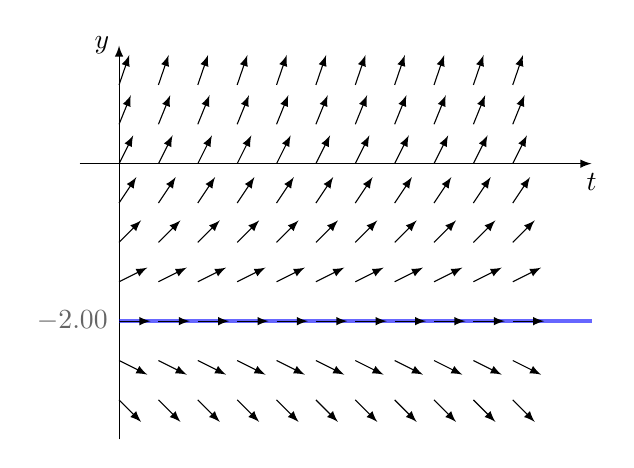
\begin{tikzpicture}
  \draw[-latex] (-0.50, 0)--(6.00, 0) node[below] {$t$};\draw[-latex] (0, -3.50)--(0, 1.50) node[left] {$y$}; \draw[ultra thick, opacity=0.6, blue] (6.00, -2.00)--(0.00, -2.00) node[left, black, fill=white] {$-2.00$};\draw[-latex] (0.00, -3.00) -- (0.28 , -3.28);\draw[-latex] (0.00, -2.50) -- (0.36 , -2.68);\draw[-latex] (0.00, -2.00) -- (0.40 , -2.00);\draw[-latex] (0.00, -1.50) -- (0.36 , -1.32);\draw[-latex] (0.00, -1.00) -- (0.28 , -0.72);\draw[-latex] (0.00, -0.50) -- (0.22 , -0.17);\draw[-latex] (0.00, 0.00) -- (0.18 , 0.36);\draw[-latex] (0.00, 0.50) -- (0.15 , 0.87);\draw[-latex] (0.00, 1.00) -- (0.13 , 1.38);\draw[-latex] (0.50, -3.00) -- (0.78 , -3.28);\draw[-latex] (0.50, -2.50) -- (0.86 , -2.68);\draw[-latex] (0.50, -2.00) -- (0.90 , -2.00);\draw[-latex] (0.50, -1.50) -- (0.86 , -1.32);\draw[-latex] (0.50, -1.00) -- (0.78 , -0.72);\draw[-latex] (0.50, -0.50) -- (0.72 , -0.17);\draw[-latex] (0.50, 0.00) -- (0.68 , 0.36);\draw[-latex] (0.50, 0.50) -- (0.65 , 0.87);\draw[-latex] (0.50, 1.00) -- (0.63 , 1.38);\draw[-latex] (1.00, -3.00) -- (1.28 , -3.28);\draw[-latex] (1.00, -2.50) -- (1.36 , -2.68);\draw[-latex] (1.00, -2.00) -- (1.40 , -2.00);\draw[-latex] (1.00, -1.50) -- (1.36 , -1.32);\draw[-latex] (1.00, -1.00) -- (1.28 , -0.72);\draw[-latex] (1.00, -0.50) -- (1.22 , -0.17);\draw[-latex] (1.00, 0.00) -- (1.18 , 0.36);\draw[-latex] (1.00, 0.50) -- (1.15 , 0.87);\draw[-latex] (1.00, 1.00) -- (1.13 , 1.38);\draw[-latex] (1.50, -3.00) -- (1.78 , -3.28);\draw[-latex] (1.50, -2.50) -- (1.86 , -2.68);\draw[-latex] (1.50, -2.00) -- (1.90 , -2.00);\draw[-latex] (1.50, -1.50) -- (1.86 , -1.32);\draw[-latex] (1.50, -1.00) -- (1.78 , -0.72);\draw[-latex] (1.50, -0.50) -- (1.72 , -0.17);\draw[-latex] (1.50, 0.00) -- (1.68 , 0.36);\draw[-latex] (1.50, 0.50) -- (1.65 , 0.87);\draw[-latex] (1.50, 1.00) -- (1.63 , 1.38);\draw[-latex] (2.00, -3.00) -- (2.28 , -3.28);\draw[-latex] (2.00, -2.50) -- (2.36 , -2.68);\draw[-latex] (2.00, -2.00) -- (2.40 , -2.00);\draw[-latex] (2.00, -1.50) -- (2.36 , -1.32);\draw[-latex] (2.00, -1.00) -- (2.28 , -0.72);\draw[-latex] (2.00, -0.50) -- (2.22 , -0.17);\draw[-latex] (2.00, 0.00) -- (2.18 , 0.36);\draw[-latex] (2.00, 0.50) -- (2.15 , 0.87);\draw[-latex] (2.00, 1.00) -- (2.13 , 1.38);\draw[-latex] (2.50, -3.00) -- (2.78 , -3.28);\draw[-latex] (2.50, -2.50) -- (2.86 , -2.68);\draw[-latex] (2.50, -2.00) -- (2.90 , -2.00);\draw[-latex] (2.50, -1.50) -- (2.86 , -1.32);\draw[-latex] (2.50, -1.00) -- (2.78 , -0.72);\draw[-latex] (2.50, -0.50) -- (2.72 , -0.17);\draw[-latex] (2.50, 0.00) -- (2.68 , 0.36);\draw[-latex] (2.50, 0.50) -- (2.65 , 0.87);\draw[-latex] (2.50, 1.00) -- (2.63 , 1.38);\draw[-latex] (3.00, -3.00) -- (3.28 , -3.28);\draw[-latex] (3.00, -2.50) -- (3.36 , -2.68);\draw[-latex] (3.00, -2.00) -- (3.40 , -2.00);\draw[-latex] (3.00, -1.50) -- (3.36 , -1.32);\draw[-latex] (3.00, -1.00) -- (3.28 , -0.72);\draw[-latex] (3.00, -0.50) -- (3.22 , -0.17);\draw[-latex] (3.00, 0.00) -- (3.18 , 0.36);\draw[-latex] (3.00, 0.50) -- (3.15 , 0.87);\draw[-latex] (3.00, 1.00) -- (3.13 , 1.38);\draw[-latex] (3.50, -3.00) -- (3.78 , -3.28);\draw[-latex] (3.50, -2.50) -- (3.86 , -2.68);\draw[-latex] (3.50, -2.00) -- (3.90 , -2.00);\draw[-latex] (3.50, -1.50) -- (3.86 , -1.32);\draw[-latex] (3.50, -1.00) -- (3.78 , -0.72);\draw[-latex] (3.50, -0.50) -- (3.72 , -0.17);\draw[-latex] (3.50, 0.00) -- (3.68 , 0.36);\draw[-latex] (3.50, 0.50) -- (3.65 , 0.87);\draw[-latex] (3.50, 1.00) -- (3.63 , 1.38);\draw[-latex] (4.00, -3.00) -- (4.28 , -3.28);\draw[-latex] (4.00, -2.50) -- (4.36 , -2.68);\draw[-latex] (4.00, -2.00) -- (4.40 , -2.00);\draw[-latex] (4.00, -1.50) -- (4.36 , -1.32);\draw[-latex] (4.00, -1.00) -- (4.28 , -0.72);\draw[-latex] (4.00, -0.50) -- (4.22 , -0.17);\draw[-latex] (4.00, 0.00) -- (4.18 , 0.36);\draw[-latex] (4.00, 0.50) -- (4.15 , 0.87);\draw[-latex] (4.00, 1.00) -- (4.13 , 1.38);\draw[-latex] (4.50, -3.00) -- (4.78 , -3.28);\draw[-latex] (4.50, -2.50) -- (4.86 , -2.68);\draw[-latex] (4.50, -2.00) -- (4.90 , -2.00);\draw[-latex] (4.50, -1.50) -- (4.86 , -1.32);\draw[-latex] (4.50, -1.00) -- (4.78 , -0.72);\draw[-latex] (4.50, -0.50) -- (4.72 , -0.17);\draw[-latex] (4.50, 0.00) -- (4.68 , 0.36);\draw[-latex] (4.50, 0.50) -- (4.65 , 0.87);\draw[-latex] (4.50, 1.00) -- (4.63 , 1.38);\draw[-latex] (5.00, -3.00) -- (5.28 , -3.28);\draw[-latex] (5.00, -2.50) -- (5.36 , -2.68);\draw[-latex] (5.00, -2.00) -- (5.40 , -2.00);\draw[-latex] (5.00, -1.50) -- (5.36 , -1.32);\draw[-latex] (5.00, -1.00) -- (5.28 , -0.72);\draw[-latex] (5.00, -0.50) -- (5.22 , -0.17);\draw[-latex] (5.00, 0.00) -- (5.18 , 0.36);\draw[-latex] (5.00, 0.50) -- (5.15 , 0.87);\draw[-latex] (5.00, 1.00) -- (5.13 , 1.38);
\end{tikzpicture}
\end{figure}

\fimSol

\noindent Em cada um dos problemas de 7 a 10, escreva uma equação diferencial da forma \(dy/dt = ay+b\) cujas soluções têm o comportamento descrito quando \(t\rightarrow \infty\).

\begin{enumerate}[resume]
    \item Todas as soluções tendem a $y = 3$.
\end{enumerate}

\iniSol

\[
\dfrac{dy}{dt} = 9 - 3y
\]
\fimSol

\begin{enumerate}[resume]
    \item Todas as soluções tendem a $y = 2/3$.
\end{enumerate}

\iniSol

\[
\dfrac{dy}{dt} = 2 - 3y
\]
\fimSol

\begin{enumerate}[resume]
    \item Todas as soluções se afastam de $y = 2$.
\end{enumerate}

\iniSol

\[
\dfrac{dy}{dt} = 4y - 8
\]
\fimSol

\begin{enumerate}[resume]
    \item Todas as soluções se afastam de  $y = 1/3$.
\end{enumerate}

\iniSol

\[
\dfrac{dy}{dt} =  3y - 1
\]
\fimSol

\noindent Nos problemas de 11 a 14, desenhe um campo de direções para a equação diferencial dada. Baseado no campo de direções, determine o comportamento de \(y\) quando \(t \rightarrow \infty\). Se esse comportamento depender do valor inicial de \(y\) quando \(t=0\), descreva essa dependência. Note que nesses problemas, as equações não são da forma \(y^\prime = ay +b\), e o comportamento das soluções é um pouco mais complicado do que o das equações no texto.

\begin{enumerate}[resume]
    \item $y^\prime = y(4-y)$
\end{enumerate}

\iniSol

Inicialmente, determinemos a solução de equilíbrio:

\begin{align*}
    y^\prime = 0 \Rightarrow y(4-y) = 0 \Rightarrow 
    \begin{cases}
      y = 0\\
      4-y =0
    \end{cases}
    \Rightarrow
    \begin{cases}
        y=0\\
        y =4
    \end{cases}
\end{align*}

Observemos que existem duas soluções de equilíbrio: \(y = 0\) e \(y = 4\), destacadas no campo de direções abaixo.

\begin{figure}[H]
\centering
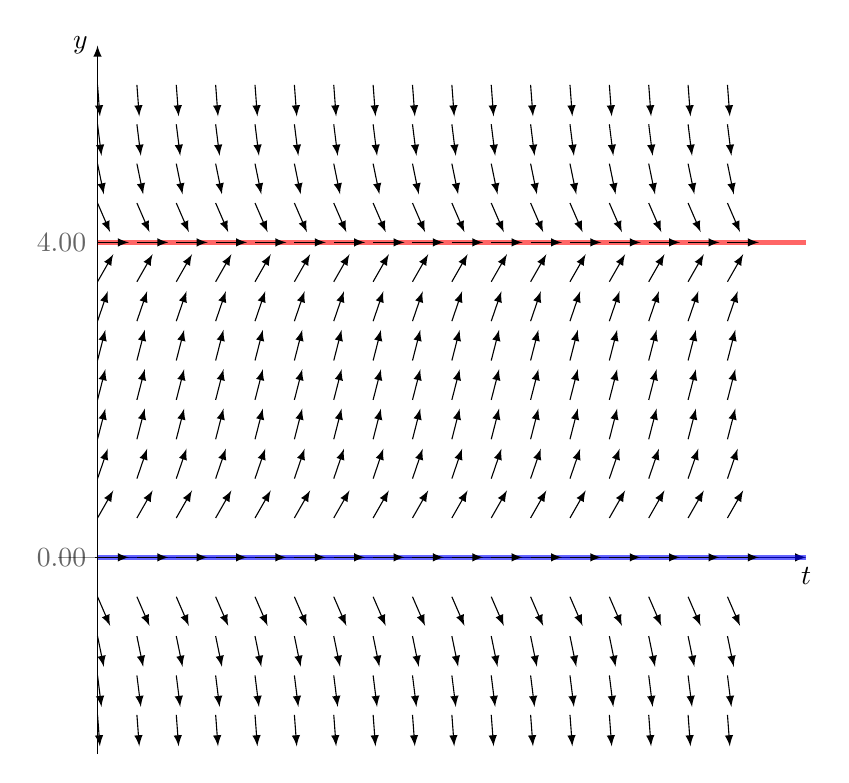
\begin{tikzpicture}
  \draw[-latex] (-0.50, 0)--(9.00, 0) node[below] {$t$};\draw[-latex] (0, -2.50)--(0, 6.50) node[left] {$y$}; \draw[ultra thick, opacity=0.6, blue] (9.00, 0.00)--(0.00, 0.00) node[left, black, fill=white] {$0.00$}; \draw[ultra thick, opacity=0.6, red] (9.00, 4.00)--(0.00, 4.00) node[left, black, fill=white] {$4.00$};\draw[-latex] (0.00, -2.00) -- (0.03 , -2.40);\draw[-latex] (0.00, -1.50) -- (0.05 , -1.90);\draw[-latex] (0.00, -1.00) -- (0.08 , -1.39);\draw[-latex] (0.00, -0.50) -- (0.16 , -0.87);\draw[-latex] (0.00, 0.00) -- (0.40 , 0.00);\draw[-latex] (0.00, 0.50) -- (0.20 , 0.85);\draw[-latex] (0.00, 1.00) -- (0.13 , 1.38);\draw[-latex] (0.00, 1.50) -- (0.10 , 1.89);\draw[-latex] (0.00, 2.00) -- (0.10 , 2.39);\draw[-latex] (0.00, 2.50) -- (0.10 , 2.89);\draw[-latex] (0.00, 3.00) -- (0.13 , 3.38);\draw[-latex] (0.00, 3.50) -- (0.20 , 3.85);\draw[-latex] (0.00, 4.00) -- (0.40 , 4.00);\draw[-latex] (0.00, 4.50) -- (0.16 , 4.13);\draw[-latex] (0.00, 5.00) -- (0.08 , 4.61);\draw[-latex] (0.00, 5.50) -- (0.05 , 5.10);\draw[-latex] (0.00, 6.00) -- (0.03 , 5.60);\draw[-latex] (0.50, -2.00) -- (0.53 , -2.40);\draw[-latex] (0.50, -1.50) -- (0.55 , -1.90);\draw[-latex] (0.50, -1.00) -- (0.58 , -1.39);\draw[-latex] (0.50, -0.50) -- (0.66 , -0.87);\draw[-latex] (0.50, 0.00) -- (0.90 , 0.00);\draw[-latex] (0.50, 0.50) -- (0.70 , 0.85);\draw[-latex] (0.50, 1.00) -- (0.63 , 1.38);\draw[-latex] (0.50, 1.50) -- (0.60 , 1.89);\draw[-latex] (0.50, 2.00) -- (0.60 , 2.39);\draw[-latex] (0.50, 2.50) -- (0.60 , 2.89);\draw[-latex] (0.50, 3.00) -- (0.63 , 3.38);\draw[-latex] (0.50, 3.50) -- (0.70 , 3.85);\draw[-latex] (0.50, 4.00) -- (0.90 , 4.00);\draw[-latex] (0.50, 4.50) -- (0.66 , 4.13);\draw[-latex] (0.50, 5.00) -- (0.58 , 4.61);\draw[-latex] (0.50, 5.50) -- (0.55 , 5.10);\draw[-latex] (0.50, 6.00) -- (0.53 , 5.60);\draw[-latex] (1.00, -2.00) -- (1.03 , -2.40);\draw[-latex] (1.00, -1.50) -- (1.05 , -1.90);\draw[-latex] (1.00, -1.00) -- (1.08 , -1.39);\draw[-latex] (1.00, -0.50) -- (1.16 , -0.87);\draw[-latex] (1.00, 0.00) -- (1.40 , 0.00);\draw[-latex] (1.00, 0.50) -- (1.20 , 0.85);\draw[-latex] (1.00, 1.00) -- (1.13 , 1.38);\draw[-latex] (1.00, 1.50) -- (1.10 , 1.89);\draw[-latex] (1.00, 2.00) -- (1.10 , 2.39);\draw[-latex] (1.00, 2.50) -- (1.10 , 2.89);\draw[-latex] (1.00, 3.00) -- (1.13 , 3.38);\draw[-latex] (1.00, 3.50) -- (1.20 , 3.85);\draw[-latex] (1.00, 4.00) -- (1.40 , 4.00);\draw[-latex] (1.00, 4.50) -- (1.16 , 4.13);\draw[-latex] (1.00, 5.00) -- (1.08 , 4.61);\draw[-latex] (1.00, 5.50) -- (1.05 , 5.10);\draw[-latex] (1.00, 6.00) -- (1.03 , 5.60);\draw[-latex] (1.50, -2.00) -- (1.53 , -2.40);\draw[-latex] (1.50, -1.50) -- (1.55 , -1.90);\draw[-latex] (1.50, -1.00) -- (1.58 , -1.39);\draw[-latex] (1.50, -0.50) -- (1.66 , -0.87);\draw[-latex] (1.50, 0.00) -- (1.90 , 0.00);\draw[-latex] (1.50, 0.50) -- (1.70 , 0.85);\draw[-latex] (1.50, 1.00) -- (1.63 , 1.38);\draw[-latex] (1.50, 1.50) -- (1.60 , 1.89);\draw[-latex] (1.50, 2.00) -- (1.60 , 2.39);\draw[-latex] (1.50, 2.50) -- (1.60 , 2.89);\draw[-latex] (1.50, 3.00) -- (1.63 , 3.38);\draw[-latex] (1.50, 3.50) -- (1.70 , 3.85);\draw[-latex] (1.50, 4.00) -- (1.90 , 4.00);\draw[-latex] (1.50, 4.50) -- (1.66 , 4.13);\draw[-latex] (1.50, 5.00) -- (1.58 , 4.61);\draw[-latex] (1.50, 5.50) -- (1.55 , 5.10);\draw[-latex] (1.50, 6.00) -- (1.53 , 5.60);\draw[-latex] (2.00, -2.00) -- (2.03 , -2.40);\draw[-latex] (2.00, -1.50) -- (2.05 , -1.90);\draw[-latex] (2.00, -1.00) -- (2.08 , -1.39);\draw[-latex] (2.00, -0.50) -- (2.16 , -0.87);\draw[-latex] (2.00, 0.00) -- (2.40 , 0.00);\draw[-latex] (2.00, 0.50) -- (2.20 , 0.85);\draw[-latex] (2.00, 1.00) -- (2.13 , 1.38);\draw[-latex] (2.00, 1.50) -- (2.10 , 1.89);\draw[-latex] (2.00, 2.00) -- (2.10 , 2.39);\draw[-latex] (2.00, 2.50) -- (2.10 , 2.89);\draw[-latex] (2.00, 3.00) -- (2.13 , 3.38);\draw[-latex] (2.00, 3.50) -- (2.20 , 3.85);\draw[-latex] (2.00, 4.00) -- (2.40 , 4.00);\draw[-latex] (2.00, 4.50) -- (2.16 , 4.13);\draw[-latex] (2.00, 5.00) -- (2.08 , 4.61);\draw[-latex] (2.00, 5.50) -- (2.05 , 5.10);\draw[-latex] (2.00, 6.00) -- (2.03 , 5.60);\draw[-latex] (2.50, -2.00) -- (2.53 , -2.40);\draw[-latex] (2.50, -1.50) -- (2.55 , -1.90);\draw[-latex] (2.50, -1.00) -- (2.58 , -1.39);\draw[-latex] (2.50, -0.50) -- (2.66 , -0.87);\draw[-latex] (2.50, 0.00) -- (2.90 , 0.00);\draw[-latex] (2.50, 0.50) -- (2.70 , 0.85);\draw[-latex] (2.50, 1.00) -- (2.63 , 1.38);\draw[-latex] (2.50, 1.50) -- (2.60 , 1.89);\draw[-latex] (2.50, 2.00) -- (2.60 , 2.39);\draw[-latex] (2.50, 2.50) -- (2.60 , 2.89);\draw[-latex] (2.50, 3.00) -- (2.63 , 3.38);\draw[-latex] (2.50, 3.50) -- (2.70 , 3.85);\draw[-latex] (2.50, 4.00) -- (2.90 , 4.00);\draw[-latex] (2.50, 4.50) -- (2.66 , 4.13);\draw[-latex] (2.50, 5.00) -- (2.58 , 4.61);\draw[-latex] (2.50, 5.50) -- (2.55 , 5.10);\draw[-latex] (2.50, 6.00) -- (2.53 , 5.60);\draw[-latex] (3.00, -2.00) -- (3.03 , -2.40);\draw[-latex] (3.00, -1.50) -- (3.05 , -1.90);\draw[-latex] (3.00, -1.00) -- (3.08 , -1.39);\draw[-latex] (3.00, -0.50) -- (3.16 , -0.87);\draw[-latex] (3.00, 0.00) -- (3.40 , 0.00);\draw[-latex] (3.00, 0.50) -- (3.20 , 0.85);\draw[-latex] (3.00, 1.00) -- (3.13 , 1.38);\draw[-latex] (3.00, 1.50) -- (3.10 , 1.89);\draw[-latex] (3.00, 2.00) -- (3.10 , 2.39);\draw[-latex] (3.00, 2.50) -- (3.10 , 2.89);\draw[-latex] (3.00, 3.00) -- (3.13 , 3.38);\draw[-latex] (3.00, 3.50) -- (3.20 , 3.85);\draw[-latex] (3.00, 4.00) -- (3.40 , 4.00);\draw[-latex] (3.00, 4.50) -- (3.16 , 4.13);\draw[-latex] (3.00, 5.00) -- (3.08 , 4.61);\draw[-latex] (3.00, 5.50) -- (3.05 , 5.10);\draw[-latex] (3.00, 6.00) -- (3.03 , 5.60);\draw[-latex] (3.50, -2.00) -- (3.53 , -2.40);\draw[-latex] (3.50, -1.50) -- (3.55 , -1.90);\draw[-latex] (3.50, -1.00) -- (3.58 , -1.39);\draw[-latex] (3.50, -0.50) -- (3.66 , -0.87);\draw[-latex] (3.50, 0.00) -- (3.90 , 0.00);\draw[-latex] (3.50, 0.50) -- (3.70 , 0.85);\draw[-latex] (3.50, 1.00) -- (3.63 , 1.38);\draw[-latex] (3.50, 1.50) -- (3.60 , 1.89);\draw[-latex] (3.50, 2.00) -- (3.60 , 2.39);\draw[-latex] (3.50, 2.50) -- (3.60 , 2.89);\draw[-latex] (3.50, 3.00) -- (3.63 , 3.38);\draw[-latex] (3.50, 3.50) -- (3.70 , 3.85);\draw[-latex] (3.50, 4.00) -- (3.90 , 4.00);\draw[-latex] (3.50, 4.50) -- (3.66 , 4.13);\draw[-latex] (3.50, 5.00) -- (3.58 , 4.61);\draw[-latex] (3.50, 5.50) -- (3.55 , 5.10);\draw[-latex] (3.50, 6.00) -- (3.53 , 5.60);\draw[-latex] (4.00, -2.00) -- (4.03 , -2.40);\draw[-latex] (4.00, -1.50) -- (4.05 , -1.90);\draw[-latex] (4.00, -1.00) -- (4.08 , -1.39);\draw[-latex] (4.00, -0.50) -- (4.16 , -0.87);\draw[-latex] (4.00, 0.00) -- (4.40 , 0.00);\draw[-latex] (4.00, 0.50) -- (4.20 , 0.85);\draw[-latex] (4.00, 1.00) -- (4.13 , 1.38);\draw[-latex] (4.00, 1.50) -- (4.10 , 1.89);\draw[-latex] (4.00, 2.00) -- (4.10 , 2.39);\draw[-latex] (4.00, 2.50) -- (4.10 , 2.89);\draw[-latex] (4.00, 3.00) -- (4.13 , 3.38);\draw[-latex] (4.00, 3.50) -- (4.20 , 3.85);\draw[-latex] (4.00, 4.00) -- (4.40 , 4.00);\draw[-latex] (4.00, 4.50) -- (4.16 , 4.13);\draw[-latex] (4.00, 5.00) -- (4.08 , 4.61);\draw[-latex] (4.00, 5.50) -- (4.05 , 5.10);\draw[-latex] (4.00, 6.00) -- (4.03 , 5.60);\draw[-latex] (4.50, -2.00) -- (4.53 , -2.40);\draw[-latex] (4.50, -1.50) -- (4.55 , -1.90);\draw[-latex] (4.50, -1.00) -- (4.58 , -1.39);\draw[-latex] (4.50, -0.50) -- (4.66 , -0.87);\draw[-latex] (4.50, 0.00) -- (4.90 , 0.00);\draw[-latex] (4.50, 0.50) -- (4.70 , 0.85);\draw[-latex] (4.50, 1.00) -- (4.63 , 1.38);\draw[-latex] (4.50, 1.50) -- (4.60 , 1.89);\draw[-latex] (4.50, 2.00) -- (4.60 , 2.39);\draw[-latex] (4.50, 2.50) -- (4.60 , 2.89);\draw[-latex] (4.50, 3.00) -- (4.63 , 3.38);\draw[-latex] (4.50, 3.50) -- (4.70 , 3.85);\draw[-latex] (4.50, 4.00) -- (4.90 , 4.00);\draw[-latex] (4.50, 4.50) -- (4.66 , 4.13);\draw[-latex] (4.50, 5.00) -- (4.58 , 4.61);\draw[-latex] (4.50, 5.50) -- (4.55 , 5.10);\draw[-latex] (4.50, 6.00) -- (4.53 , 5.60);\draw[-latex] (5.00, -2.00) -- (5.03 , -2.40);\draw[-latex] (5.00, -1.50) -- (5.05 , -1.90);\draw[-latex] (5.00, -1.00) -- (5.08 , -1.39);\draw[-latex] (5.00, -0.50) -- (5.16 , -0.87);\draw[-latex] (5.00, 0.00) -- (5.40 , 0.00);\draw[-latex] (5.00, 0.50) -- (5.20 , 0.85);\draw[-latex] (5.00, 1.00) -- (5.13 , 1.38);\draw[-latex] (5.00, 1.50) -- (5.10 , 1.89);\draw[-latex] (5.00, 2.00) -- (5.10 , 2.39);\draw[-latex] (5.00, 2.50) -- (5.10 , 2.89);\draw[-latex] (5.00, 3.00) -- (5.13 , 3.38);\draw[-latex] (5.00, 3.50) -- (5.20 , 3.85);\draw[-latex] (5.00, 4.00) -- (5.40 , 4.00);\draw[-latex] (5.00, 4.50) -- (5.16 , 4.13);\draw[-latex] (5.00, 5.00) -- (5.08 , 4.61);\draw[-latex] (5.00, 5.50) -- (5.05 , 5.10);\draw[-latex] (5.00, 6.00) -- (5.03 , 5.60);\draw[-latex] (5.50, -2.00) -- (5.53 , -2.40);\draw[-latex] (5.50, -1.50) -- (5.55 , -1.90);\draw[-latex] (5.50, -1.00) -- (5.58 , -1.39);\draw[-latex] (5.50, -0.50) -- (5.66 , -0.87);\draw[-latex] (5.50, 0.00) -- (5.90 , 0.00);\draw[-latex] (5.50, 0.50) -- (5.70 , 0.85);\draw[-latex] (5.50, 1.00) -- (5.63 , 1.38);\draw[-latex] (5.50, 1.50) -- (5.60 , 1.89);\draw[-latex] (5.50, 2.00) -- (5.60 , 2.39);\draw[-latex] (5.50, 2.50) -- (5.60 , 2.89);\draw[-latex] (5.50, 3.00) -- (5.63 , 3.38);\draw[-latex] (5.50, 3.50) -- (5.70 , 3.85);\draw[-latex] (5.50, 4.00) -- (5.90 , 4.00);\draw[-latex] (5.50, 4.50) -- (5.66 , 4.13);\draw[-latex] (5.50, 5.00) -- (5.58 , 4.61);\draw[-latex] (5.50, 5.50) -- (5.55 , 5.10);\draw[-latex] (5.50, 6.00) -- (5.53 , 5.60);\draw[-latex] (6.00, -2.00) -- (6.03 , -2.40);\draw[-latex] (6.00, -1.50) -- (6.05 , -1.90);\draw[-latex] (6.00, -1.00) -- (6.08 , -1.39);\draw[-latex] (6.00, -0.50) -- (6.16 , -0.87);\draw[-latex] (6.00, 0.00) -- (6.40 , 0.00);\draw[-latex] (6.00, 0.50) -- (6.20 , 0.85);\draw[-latex] (6.00, 1.00) -- (6.13 , 1.38);\draw[-latex] (6.00, 1.50) -- (6.10 , 1.89);\draw[-latex] (6.00, 2.00) -- (6.10 , 2.39);\draw[-latex] (6.00, 2.50) -- (6.10 , 2.89);\draw[-latex] (6.00, 3.00) -- (6.13 , 3.38);\draw[-latex] (6.00, 3.50) -- (6.20 , 3.85);\draw[-latex] (6.00, 4.00) -- (6.40 , 4.00);\draw[-latex] (6.00, 4.50) -- (6.16 , 4.13);\draw[-latex] (6.00, 5.00) -- (6.08 , 4.61);\draw[-latex] (6.00, 5.50) -- (6.05 , 5.10);\draw[-latex] (6.00, 6.00) -- (6.03 , 5.60);\draw[-latex] (6.50, -2.00) -- (6.53 , -2.40);\draw[-latex] (6.50, -1.50) -- (6.55 , -1.90);\draw[-latex] (6.50, -1.00) -- (6.58 , -1.39);\draw[-latex] (6.50, -0.50) -- (6.66 , -0.87);\draw[-latex] (6.50, 0.00) -- (6.90 , 0.00);\draw[-latex] (6.50, 0.50) -- (6.70 , 0.85);\draw[-latex] (6.50, 1.00) -- (6.63 , 1.38);\draw[-latex] (6.50, 1.50) -- (6.60 , 1.89);\draw[-latex] (6.50, 2.00) -- (6.60 , 2.39);\draw[-latex] (6.50, 2.50) -- (6.60 , 2.89);\draw[-latex] (6.50, 3.00) -- (6.63 , 3.38);\draw[-latex] (6.50, 3.50) -- (6.70 , 3.85);\draw[-latex] (6.50, 4.00) -- (6.90 , 4.00);\draw[-latex] (6.50, 4.50) -- (6.66 , 4.13);\draw[-latex] (6.50, 5.00) -- (6.58 , 4.61);\draw[-latex] (6.50, 5.50) -- (6.55 , 5.10);\draw[-latex] (6.50, 6.00) -- (6.53 , 5.60);\draw[-latex] (7.00, -2.00) -- (7.03 , -2.40);\draw[-latex] (7.00, -1.50) -- (7.05 , -1.90);\draw[-latex] (7.00, -1.00) -- (7.08 , -1.39);\draw[-latex] (7.00, -0.50) -- (7.16 , -0.87);\draw[-latex] (7.00, 0.00) -- (7.40 , 0.00);\draw[-latex] (7.00, 0.50) -- (7.20 , 0.85);\draw[-latex] (7.00, 1.00) -- (7.13 , 1.38);\draw[-latex] (7.00, 1.50) -- (7.10 , 1.89);\draw[-latex] (7.00, 2.00) -- (7.10 , 2.39);\draw[-latex] (7.00, 2.50) -- (7.10 , 2.89);\draw[-latex] (7.00, 3.00) -- (7.13 , 3.38);\draw[-latex] (7.00, 3.50) -- (7.20 , 3.85);\draw[-latex] (7.00, 4.00) -- (7.40 , 4.00);\draw[-latex] (7.00, 4.50) -- (7.16 , 4.13);\draw[-latex] (7.00, 5.00) -- (7.08 , 4.61);\draw[-latex] (7.00, 5.50) -- (7.05 , 5.10);\draw[-latex] (7.00, 6.00) -- (7.03 , 5.60);\draw[-latex] (7.50, -2.00) -- (7.53 , -2.40);\draw[-latex] (7.50, -1.50) -- (7.55 , -1.90);\draw[-latex] (7.50, -1.00) -- (7.58 , -1.39);\draw[-latex] (7.50, -0.50) -- (7.66 , -0.87);\draw[-latex] (7.50, 0.00) -- (7.90 , 0.00);\draw[-latex] (7.50, 0.50) -- (7.70 , 0.85);\draw[-latex] (7.50, 1.00) -- (7.63 , 1.38);\draw[-latex] (7.50, 1.50) -- (7.60 , 1.89);\draw[-latex] (7.50, 2.00) -- (7.60 , 2.39);\draw[-latex] (7.50, 2.50) -- (7.60 , 2.89);\draw[-latex] (7.50, 3.00) -- (7.63 , 3.38);\draw[-latex] (7.50, 3.50) -- (7.70 , 3.85);\draw[-latex] (7.50, 4.00) -- (7.90 , 4.00);\draw[-latex] (7.50, 4.50) -- (7.66 , 4.13);\draw[-latex] (7.50, 5.00) -- (7.58 , 4.61);\draw[-latex] (7.50, 5.50) -- (7.55 , 5.10);\draw[-latex] (7.50, 6.00) -- (7.53 , 5.60);\draw[-latex] (8.00, -2.00) -- (8.03 , -2.40);\draw[-latex] (8.00, -1.50) -- (8.05 , -1.90);\draw[-latex] (8.00, -1.00) -- (8.08 , -1.39);\draw[-latex] (8.00, -0.50) -- (8.16 , -0.87);\draw[-latex] (8.00, 0.00) -- (8.40 , 0.00);\draw[-latex] (8.00, 0.50) -- (8.20 , 0.85);\draw[-latex] (8.00, 1.00) -- (8.13 , 1.38);\draw[-latex] (8.00, 1.50) -- (8.10 , 1.89);\draw[-latex] (8.00, 2.00) -- (8.10 , 2.39);\draw[-latex] (8.00, 2.50) -- (8.10 , 2.89);\draw[-latex] (8.00, 3.00) -- (8.13 , 3.38);\draw[-latex] (8.00, 3.50) -- (8.20 , 3.85);\draw[-latex] (8.00, 4.00) -- (8.40 , 4.00);\draw[-latex] (8.00, 4.50) -- (8.16 , 4.13);\draw[-latex] (8.00, 5.00) -- (8.08 , 4.61);\draw[-latex] (8.00, 5.50) -- (8.05 , 5.10);\draw[-latex] (8.00, 6.00) -- (8.03 , 5.60);
\end{tikzpicture}
\end{figure}

Como ilustra o campo de direções acima, o comportamento das soluções quando \(t \rightarrow \infty\) depende do valor inicial de \(y\) em \(t = 0\). De fato, seja a condição inicial \(y_0 = y(t=0)\). Então

\begin{itemize}
 \item Soluções em que $y_0 < 0$ afastam-se da solução de equilíbrio $y = 0$. Ou seja,   $\displaystyle \lim_{t \rightarrow \infty} y = -\infty$ . 
 \item Soluções em que $y_0 > 4$ tendem  à solução de equilíbrio $y = 4$. Ou seja,   $\displaystyle \lim_{t \rightarrow \infty} y = 4$ .
 \item Soluções em que $0 < y_0 < 4$ afastam-se da solução de equilíbrio $y = 0$ e tendem à solução $y = 4$. Ou seja,   $\displaystyle \lim_{t \rightarrow \infty} y = 4$ .
\end{itemize}

\fimSol

\begin{enumerate}[resume]
    \item $y^\prime = -y(5-y)$
\end{enumerate}

\iniSol

Inicialmente, determinemos a solução de equilíbrio:

\begin{align*}
    y^\prime = 0 \Rightarrow -y(5-y) = 0 \Rightarrow 
    \begin{cases}
      -y = 0\\
      5-y =0
    \end{cases}
    \Rightarrow
    \begin{cases}
        y=0\\
        y =5
    \end{cases}
\end{align*}

Observemos que existem duas soluções de equilíbrio: \(y = 0\) e \(y = 5\), destacadas no campo de direções abaixo.

\begin{figure}[H]
\centering
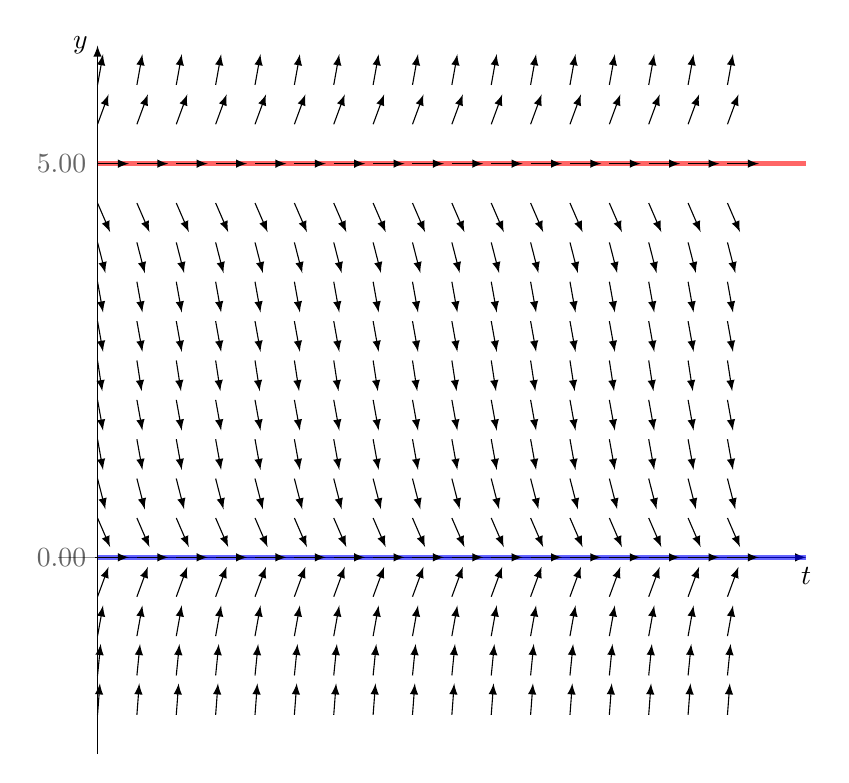
\begin{tikzpicture}
  \draw[-latex] (-0.50, 0)--(9.00, 0) node[below] {$t$};\draw[-latex] (0, -2.50)--(0, 6.50) node[left] {$y$}; \draw[ultra thick, opacity=0.6, blue] (9.00, 0.00)--(0.00, 0.00) node[left, black, fill=white] {$0.00$}; \draw[ultra thick, opacity=0.6, red] (9.00, 5.00)--(0.00, 5.00) node[left, black, fill=white] {$5.00$};\draw[-latex] (0.00, -2.00) -- (0.03 , -1.60);\draw[-latex] (0.00, -1.50) -- (0.04 , -1.10);\draw[-latex] (0.00, -1.00) -- (0.07 , -0.61);\draw[-latex] (0.00, -0.50) -- (0.14 , -0.12);\draw[-latex] (0.00, 0.00) -- (0.40 , 0.00);\draw[-latex] (0.00, 0.50) -- (0.16 , 0.13);\draw[-latex] (0.00, 1.00) -- (0.10 , 0.61);\draw[-latex] (0.00, 1.50) -- (0.07 , 1.11);\draw[-latex] (0.00, 2.00) -- (0.07 , 1.61);\draw[-latex] (0.00, 2.50) -- (0.06 , 2.11);\draw[-latex] (0.00, 3.00) -- (0.07 , 2.61);\draw[-latex] (0.00, 3.50) -- (0.07 , 3.11);\draw[-latex] (0.00, 4.00) -- (0.10 , 3.61);\draw[-latex] (0.00, 4.50) -- (0.16 , 4.13);\draw[-latex] (0.00, 5.00) -- (0.40 , 5.00);\draw[-latex] (0.00, 5.50) -- (0.14 , 5.88);\draw[-latex] (0.00, 6.00) -- (0.07 , 6.39);\draw[-latex] (0.50, -2.00) -- (0.53 , -1.60);\draw[-latex] (0.50, -1.50) -- (0.54 , -1.10);\draw[-latex] (0.50, -1.00) -- (0.57 , -0.61);\draw[-latex] (0.50, -0.50) -- (0.64 , -0.12);\draw[-latex] (0.50, 0.00) -- (0.90 , 0.00);\draw[-latex] (0.50, 0.50) -- (0.66 , 0.13);\draw[-latex] (0.50, 1.00) -- (0.60 , 0.61);\draw[-latex] (0.50, 1.50) -- (0.57 , 1.11);\draw[-latex] (0.50, 2.00) -- (0.57 , 1.61);\draw[-latex] (0.50, 2.50) -- (0.56 , 2.11);\draw[-latex] (0.50, 3.00) -- (0.57 , 2.61);\draw[-latex] (0.50, 3.50) -- (0.57 , 3.11);\draw[-latex] (0.50, 4.00) -- (0.60 , 3.61);\draw[-latex] (0.50, 4.50) -- (0.66 , 4.13);\draw[-latex] (0.50, 5.00) -- (0.90 , 5.00);\draw[-latex] (0.50, 5.50) -- (0.64 , 5.88);\draw[-latex] (0.50, 6.00) -- (0.57 , 6.39);\draw[-latex] (1.00, -2.00) -- (1.03 , -1.60);\draw[-latex] (1.00, -1.50) -- (1.04 , -1.10);\draw[-latex] (1.00, -1.00) -- (1.07 , -0.61);\draw[-latex] (1.00, -0.50) -- (1.14 , -0.12);\draw[-latex] (1.00, 0.00) -- (1.40 , 0.00);\draw[-latex] (1.00, 0.50) -- (1.16 , 0.13);\draw[-latex] (1.00, 1.00) -- (1.10 , 0.61);\draw[-latex] (1.00, 1.50) -- (1.07 , 1.11);\draw[-latex] (1.00, 2.00) -- (1.07 , 1.61);\draw[-latex] (1.00, 2.50) -- (1.06 , 2.11);\draw[-latex] (1.00, 3.00) -- (1.07 , 2.61);\draw[-latex] (1.00, 3.50) -- (1.07 , 3.11);\draw[-latex] (1.00, 4.00) -- (1.10 , 3.61);\draw[-latex] (1.00, 4.50) -- (1.16 , 4.13);\draw[-latex] (1.00, 5.00) -- (1.40 , 5.00);\draw[-latex] (1.00, 5.50) -- (1.14 , 5.88);\draw[-latex] (1.00, 6.00) -- (1.07 , 6.39);\draw[-latex] (1.50, -2.00) -- (1.53 , -1.60);\draw[-latex] (1.50, -1.50) -- (1.54 , -1.10);\draw[-latex] (1.50, -1.00) -- (1.57 , -0.61);\draw[-latex] (1.50, -0.50) -- (1.64 , -0.12);\draw[-latex] (1.50, 0.00) -- (1.90 , 0.00);\draw[-latex] (1.50, 0.50) -- (1.66 , 0.13);\draw[-latex] (1.50, 1.00) -- (1.60 , 0.61);\draw[-latex] (1.50, 1.50) -- (1.57 , 1.11);\draw[-latex] (1.50, 2.00) -- (1.57 , 1.61);\draw[-latex] (1.50, 2.50) -- (1.56 , 2.11);\draw[-latex] (1.50, 3.00) -- (1.57 , 2.61);\draw[-latex] (1.50, 3.50) -- (1.57 , 3.11);\draw[-latex] (1.50, 4.00) -- (1.60 , 3.61);\draw[-latex] (1.50, 4.50) -- (1.66 , 4.13);\draw[-latex] (1.50, 5.00) -- (1.90 , 5.00);\draw[-latex] (1.50, 5.50) -- (1.64 , 5.88);\draw[-latex] (1.50, 6.00) -- (1.57 , 6.39);\draw[-latex] (2.00, -2.00) -- (2.03 , -1.60);\draw[-latex] (2.00, -1.50) -- (2.04 , -1.10);\draw[-latex] (2.00, -1.00) -- (2.07 , -0.61);\draw[-latex] (2.00, -0.50) -- (2.14 , -0.12);\draw[-latex] (2.00, 0.00) -- (2.40 , 0.00);\draw[-latex] (2.00, 0.50) -- (2.16 , 0.13);\draw[-latex] (2.00, 1.00) -- (2.10 , 0.61);\draw[-latex] (2.00, 1.50) -- (2.07 , 1.11);\draw[-latex] (2.00, 2.00) -- (2.07 , 1.61);\draw[-latex] (2.00, 2.50) -- (2.06 , 2.11);\draw[-latex] (2.00, 3.00) -- (2.07 , 2.61);\draw[-latex] (2.00, 3.50) -- (2.07 , 3.11);\draw[-latex] (2.00, 4.00) -- (2.10 , 3.61);\draw[-latex] (2.00, 4.50) -- (2.16 , 4.13);\draw[-latex] (2.00, 5.00) -- (2.40 , 5.00);\draw[-latex] (2.00, 5.50) -- (2.14 , 5.88);\draw[-latex] (2.00, 6.00) -- (2.07 , 6.39);\draw[-latex] (2.50, -2.00) -- (2.53 , -1.60);\draw[-latex] (2.50, -1.50) -- (2.54 , -1.10);\draw[-latex] (2.50, -1.00) -- (2.57 , -0.61);\draw[-latex] (2.50, -0.50) -- (2.64 , -0.12);\draw[-latex] (2.50, 0.00) -- (2.90 , 0.00);\draw[-latex] (2.50, 0.50) -- (2.66 , 0.13);\draw[-latex] (2.50, 1.00) -- (2.60 , 0.61);\draw[-latex] (2.50, 1.50) -- (2.57 , 1.11);\draw[-latex] (2.50, 2.00) -- (2.57 , 1.61);\draw[-latex] (2.50, 2.50) -- (2.56 , 2.11);\draw[-latex] (2.50, 3.00) -- (2.57 , 2.61);\draw[-latex] (2.50, 3.50) -- (2.57 , 3.11);\draw[-latex] (2.50, 4.00) -- (2.60 , 3.61);\draw[-latex] (2.50, 4.50) -- (2.66 , 4.13);\draw[-latex] (2.50, 5.00) -- (2.90 , 5.00);\draw[-latex] (2.50, 5.50) -- (2.64 , 5.88);\draw[-latex] (2.50, 6.00) -- (2.57 , 6.39);\draw[-latex] (3.00, -2.00) -- (3.03 , -1.60);\draw[-latex] (3.00, -1.50) -- (3.04 , -1.10);\draw[-latex] (3.00, -1.00) -- (3.07 , -0.61);\draw[-latex] (3.00, -0.50) -- (3.14 , -0.12);\draw[-latex] (3.00, 0.00) -- (3.40 , 0.00);\draw[-latex] (3.00, 0.50) -- (3.16 , 0.13);\draw[-latex] (3.00, 1.00) -- (3.10 , 0.61);\draw[-latex] (3.00, 1.50) -- (3.07 , 1.11);\draw[-latex] (3.00, 2.00) -- (3.07 , 1.61);\draw[-latex] (3.00, 2.50) -- (3.06 , 2.11);\draw[-latex] (3.00, 3.00) -- (3.07 , 2.61);\draw[-latex] (3.00, 3.50) -- (3.07 , 3.11);\draw[-latex] (3.00, 4.00) -- (3.10 , 3.61);\draw[-latex] (3.00, 4.50) -- (3.16 , 4.13);\draw[-latex] (3.00, 5.00) -- (3.40 , 5.00);\draw[-latex] (3.00, 5.50) -- (3.14 , 5.88);\draw[-latex] (3.00, 6.00) -- (3.07 , 6.39);\draw[-latex] (3.50, -2.00) -- (3.53 , -1.60);\draw[-latex] (3.50, -1.50) -- (3.54 , -1.10);\draw[-latex] (3.50, -1.00) -- (3.57 , -0.61);\draw[-latex] (3.50, -0.50) -- (3.64 , -0.12);\draw[-latex] (3.50, 0.00) -- (3.90 , 0.00);\draw[-latex] (3.50, 0.50) -- (3.66 , 0.13);\draw[-latex] (3.50, 1.00) -- (3.60 , 0.61);\draw[-latex] (3.50, 1.50) -- (3.57 , 1.11);\draw[-latex] (3.50, 2.00) -- (3.57 , 1.61);\draw[-latex] (3.50, 2.50) -- (3.56 , 2.11);\draw[-latex] (3.50, 3.00) -- (3.57 , 2.61);\draw[-latex] (3.50, 3.50) -- (3.57 , 3.11);\draw[-latex] (3.50, 4.00) -- (3.60 , 3.61);\draw[-latex] (3.50, 4.50) -- (3.66 , 4.13);\draw[-latex] (3.50, 5.00) -- (3.90 , 5.00);\draw[-latex] (3.50, 5.50) -- (3.64 , 5.88);\draw[-latex] (3.50, 6.00) -- (3.57 , 6.39);\draw[-latex] (4.00, -2.00) -- (4.03 , -1.60);\draw[-latex] (4.00, -1.50) -- (4.04 , -1.10);\draw[-latex] (4.00, -1.00) -- (4.07 , -0.61);\draw[-latex] (4.00, -0.50) -- (4.14 , -0.12);\draw[-latex] (4.00, 0.00) -- (4.40 , 0.00);\draw[-latex] (4.00, 0.50) -- (4.16 , 0.13);\draw[-latex] (4.00, 1.00) -- (4.10 , 0.61);\draw[-latex] (4.00, 1.50) -- (4.07 , 1.11);\draw[-latex] (4.00, 2.00) -- (4.07 , 1.61);\draw[-latex] (4.00, 2.50) -- (4.06 , 2.11);\draw[-latex] (4.00, 3.00) -- (4.07 , 2.61);\draw[-latex] (4.00, 3.50) -- (4.07 , 3.11);\draw[-latex] (4.00, 4.00) -- (4.10 , 3.61);\draw[-latex] (4.00, 4.50) -- (4.16 , 4.13);\draw[-latex] (4.00, 5.00) -- (4.40 , 5.00);\draw[-latex] (4.00, 5.50) -- (4.14 , 5.88);\draw[-latex] (4.00, 6.00) -- (4.07 , 6.39);\draw[-latex] (4.50, -2.00) -- (4.53 , -1.60);\draw[-latex] (4.50, -1.50) -- (4.54 , -1.10);\draw[-latex] (4.50, -1.00) -- (4.57 , -0.61);\draw[-latex] (4.50, -0.50) -- (4.64 , -0.12);\draw[-latex] (4.50, 0.00) -- (4.90 , 0.00);\draw[-latex] (4.50, 0.50) -- (4.66 , 0.13);\draw[-latex] (4.50, 1.00) -- (4.60 , 0.61);\draw[-latex] (4.50, 1.50) -- (4.57 , 1.11);\draw[-latex] (4.50, 2.00) -- (4.57 , 1.61);\draw[-latex] (4.50, 2.50) -- (4.56 , 2.11);\draw[-latex] (4.50, 3.00) -- (4.57 , 2.61);\draw[-latex] (4.50, 3.50) -- (4.57 , 3.11);\draw[-latex] (4.50, 4.00) -- (4.60 , 3.61);\draw[-latex] (4.50, 4.50) -- (4.66 , 4.13);\draw[-latex] (4.50, 5.00) -- (4.90 , 5.00);\draw[-latex] (4.50, 5.50) -- (4.64 , 5.88);\draw[-latex] (4.50, 6.00) -- (4.57 , 6.39);\draw[-latex] (5.00, -2.00) -- (5.03 , -1.60);\draw[-latex] (5.00, -1.50) -- (5.04 , -1.10);\draw[-latex] (5.00, -1.00) -- (5.07 , -0.61);\draw[-latex] (5.00, -0.50) -- (5.14 , -0.12);\draw[-latex] (5.00, 0.00) -- (5.40 , 0.00);\draw[-latex] (5.00, 0.50) -- (5.16 , 0.13);\draw[-latex] (5.00, 1.00) -- (5.10 , 0.61);\draw[-latex] (5.00, 1.50) -- (5.07 , 1.11);\draw[-latex] (5.00, 2.00) -- (5.07 , 1.61);\draw[-latex] (5.00, 2.50) -- (5.06 , 2.11);\draw[-latex] (5.00, 3.00) -- (5.07 , 2.61);\draw[-latex] (5.00, 3.50) -- (5.07 , 3.11);\draw[-latex] (5.00, 4.00) -- (5.10 , 3.61);\draw[-latex] (5.00, 4.50) -- (5.16 , 4.13);\draw[-latex] (5.00, 5.00) -- (5.40 , 5.00);\draw[-latex] (5.00, 5.50) -- (5.14 , 5.88);\draw[-latex] (5.00, 6.00) -- (5.07 , 6.39);\draw[-latex] (5.50, -2.00) -- (5.53 , -1.60);\draw[-latex] (5.50, -1.50) -- (5.54 , -1.10);\draw[-latex] (5.50, -1.00) -- (5.57 , -0.61);\draw[-latex] (5.50, -0.50) -- (5.64 , -0.12);\draw[-latex] (5.50, 0.00) -- (5.90 , 0.00);\draw[-latex] (5.50, 0.50) -- (5.66 , 0.13);\draw[-latex] (5.50, 1.00) -- (5.60 , 0.61);\draw[-latex] (5.50, 1.50) -- (5.57 , 1.11);\draw[-latex] (5.50, 2.00) -- (5.57 , 1.61);\draw[-latex] (5.50, 2.50) -- (5.56 , 2.11);\draw[-latex] (5.50, 3.00) -- (5.57 , 2.61);\draw[-latex] (5.50, 3.50) -- (5.57 , 3.11);\draw[-latex] (5.50, 4.00) -- (5.60 , 3.61);\draw[-latex] (5.50, 4.50) -- (5.66 , 4.13);\draw[-latex] (5.50, 5.00) -- (5.90 , 5.00);\draw[-latex] (5.50, 5.50) -- (5.64 , 5.88);\draw[-latex] (5.50, 6.00) -- (5.57 , 6.39);\draw[-latex] (6.00, -2.00) -- (6.03 , -1.60);\draw[-latex] (6.00, -1.50) -- (6.04 , -1.10);\draw[-latex] (6.00, -1.00) -- (6.07 , -0.61);\draw[-latex] (6.00, -0.50) -- (6.14 , -0.12);\draw[-latex] (6.00, 0.00) -- (6.40 , 0.00);\draw[-latex] (6.00, 0.50) -- (6.16 , 0.13);\draw[-latex] (6.00, 1.00) -- (6.10 , 0.61);\draw[-latex] (6.00, 1.50) -- (6.07 , 1.11);\draw[-latex] (6.00, 2.00) -- (6.07 , 1.61);\draw[-latex] (6.00, 2.50) -- (6.06 , 2.11);\draw[-latex] (6.00, 3.00) -- (6.07 , 2.61);\draw[-latex] (6.00, 3.50) -- (6.07 , 3.11);\draw[-latex] (6.00, 4.00) -- (6.10 , 3.61);\draw[-latex] (6.00, 4.50) -- (6.16 , 4.13);\draw[-latex] (6.00, 5.00) -- (6.40 , 5.00);\draw[-latex] (6.00, 5.50) -- (6.14 , 5.88);\draw[-latex] (6.00, 6.00) -- (6.07 , 6.39);\draw[-latex] (6.50, -2.00) -- (6.53 , -1.60);\draw[-latex] (6.50, -1.50) -- (6.54 , -1.10);\draw[-latex] (6.50, -1.00) -- (6.57 , -0.61);\draw[-latex] (6.50, -0.50) -- (6.64 , -0.12);\draw[-latex] (6.50, 0.00) -- (6.90 , 0.00);\draw[-latex] (6.50, 0.50) -- (6.66 , 0.13);\draw[-latex] (6.50, 1.00) -- (6.60 , 0.61);\draw[-latex] (6.50, 1.50) -- (6.57 , 1.11);\draw[-latex] (6.50, 2.00) -- (6.57 , 1.61);\draw[-latex] (6.50, 2.50) -- (6.56 , 2.11);\draw[-latex] (6.50, 3.00) -- (6.57 , 2.61);\draw[-latex] (6.50, 3.50) -- (6.57 , 3.11);\draw[-latex] (6.50, 4.00) -- (6.60 , 3.61);\draw[-latex] (6.50, 4.50) -- (6.66 , 4.13);\draw[-latex] (6.50, 5.00) -- (6.90 , 5.00);\draw[-latex] (6.50, 5.50) -- (6.64 , 5.88);\draw[-latex] (6.50, 6.00) -- (6.57 , 6.39);\draw[-latex] (7.00, -2.00) -- (7.03 , -1.60);\draw[-latex] (7.00, -1.50) -- (7.04 , -1.10);\draw[-latex] (7.00, -1.00) -- (7.07 , -0.61);\draw[-latex] (7.00, -0.50) -- (7.14 , -0.12);\draw[-latex] (7.00, 0.00) -- (7.40 , 0.00);\draw[-latex] (7.00, 0.50) -- (7.16 , 0.13);\draw[-latex] (7.00, 1.00) -- (7.10 , 0.61);\draw[-latex] (7.00, 1.50) -- (7.07 , 1.11);\draw[-latex] (7.00, 2.00) -- (7.07 , 1.61);\draw[-latex] (7.00, 2.50) -- (7.06 , 2.11);\draw[-latex] (7.00, 3.00) -- (7.07 , 2.61);\draw[-latex] (7.00, 3.50) -- (7.07 , 3.11);\draw[-latex] (7.00, 4.00) -- (7.10 , 3.61);\draw[-latex] (7.00, 4.50) -- (7.16 , 4.13);\draw[-latex] (7.00, 5.00) -- (7.40 , 5.00);\draw[-latex] (7.00, 5.50) -- (7.14 , 5.88);\draw[-latex] (7.00, 6.00) -- (7.07 , 6.39);\draw[-latex] (7.50, -2.00) -- (7.53 , -1.60);\draw[-latex] (7.50, -1.50) -- (7.54 , -1.10);\draw[-latex] (7.50, -1.00) -- (7.57 , -0.61);\draw[-latex] (7.50, -0.50) -- (7.64 , -0.12);\draw[-latex] (7.50, 0.00) -- (7.90 , 0.00);\draw[-latex] (7.50, 0.50) -- (7.66 , 0.13);\draw[-latex] (7.50, 1.00) -- (7.60 , 0.61);\draw[-latex] (7.50, 1.50) -- (7.57 , 1.11);\draw[-latex] (7.50, 2.00) -- (7.57 , 1.61);\draw[-latex] (7.50, 2.50) -- (7.56 , 2.11);\draw[-latex] (7.50, 3.00) -- (7.57 , 2.61);\draw[-latex] (7.50, 3.50) -- (7.57 , 3.11);\draw[-latex] (7.50, 4.00) -- (7.60 , 3.61);\draw[-latex] (7.50, 4.50) -- (7.66 , 4.13);\draw[-latex] (7.50, 5.00) -- (7.90 , 5.00);\draw[-latex] (7.50, 5.50) -- (7.64 , 5.88);\draw[-latex] (7.50, 6.00) -- (7.57 , 6.39);\draw[-latex] (8.00, -2.00) -- (8.03 , -1.60);\draw[-latex] (8.00, -1.50) -- (8.04 , -1.10);\draw[-latex] (8.00, -1.00) -- (8.07 , -0.61);\draw[-latex] (8.00, -0.50) -- (8.14 , -0.12);\draw[-latex] (8.00, 0.00) -- (8.40 , 0.00);\draw[-latex] (8.00, 0.50) -- (8.16 , 0.13);\draw[-latex] (8.00, 1.00) -- (8.10 , 0.61);\draw[-latex] (8.00, 1.50) -- (8.07 , 1.11);\draw[-latex] (8.00, 2.00) -- (8.07 , 1.61);\draw[-latex] (8.00, 2.50) -- (8.06 , 2.11);\draw[-latex] (8.00, 3.00) -- (8.07 , 2.61);\draw[-latex] (8.00, 3.50) -- (8.07 , 3.11);\draw[-latex] (8.00, 4.00) -- (8.10 , 3.61);\draw[-latex] (8.00, 4.50) -- (8.16 , 4.13);\draw[-latex] (8.00, 5.00) -- (8.40 , 5.00);\draw[-latex] (8.00, 5.50) -- (8.14 , 5.88);\draw[-latex] (8.00, 6.00) -- (8.07 , 6.39);
\end{tikzpicture}
\end{figure}

Como ilustra o campo de direções acima, o comportamento das soluções quando \(t \rightarrow \infty\) depende do valor inicial de \(y\) em \(t = 0\). De fato, seja a condição inicial \(y_0 = y(t=0)\). Então

\begin{itemize}
 \item Soluções em que $y_0 < 0$ tendem à solução de equilíbrio $y = 0$. Ou seja,   $\displaystyle \lim_{t \rightarrow \infty} y = 0$ . 
 \item Soluções em que $y_0 > 5$ afastam-se da solução de equilíbrio $y = 5$. Ou seja,   $\displaystyle \lim_{t \rightarrow \infty} y = \infty$.
 \item Soluções em que $0 < y_0 < 5$ afastam-se da solução de equilíbrio $y = 5$ e tendem à solução $y = 0$. Ou seja,   $\displaystyle \lim_{t \rightarrow \infty} y = 0$ .
\end{itemize}

\fimSol

\begin{enumerate}[resume]
    \item $y^\prime = y^2$
\end{enumerate}

\iniSol

Inicialmente, determinemos a solução de equilíbrio:

\begin{align*}
    y^\prime = 0 \Rightarrow y^2 = 0 \Rightarrow  y = 0
\end{align*}

Observemos que existe uma solução de equilíbrio: \(y = 0\), destacada no campo de direções abaixo.

\begin{figure}[H]
\centering
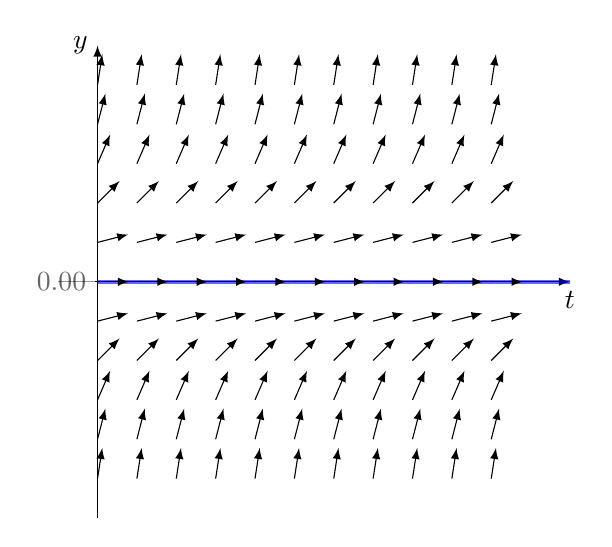
\begin{tikzpicture}
  \draw[-latex] (-0.50, 0)--(6.00, 0) node[below] {$t$};\draw[-latex] (0, -3.00)--(0, 3.00) node[left] {$y$}; \draw[ultra thick, opacity=0.6, blue] (6.00, 0.00)--(0.00, 0.00) node[left, black, fill=white] {$0.00$};\draw[-latex] (0.00, -2.50) -- (0.06 , -2.11);\draw[-latex] (0.00, -2.00) -- (0.10 , -1.61);\draw[-latex] (0.00, -1.50) -- (0.16 , -1.13);\draw[-latex] (0.00, -1.00) -- (0.28 , -0.72);\draw[-latex] (0.00, -0.50) -- (0.39 , -0.40);\draw[-latex] (0.00, 0.00) -- (0.40 , 0.00);\draw[-latex] (0.00, 0.50) -- (0.39 , 0.60);\draw[-latex] (0.00, 1.00) -- (0.28 , 1.28);\draw[-latex] (0.00, 1.50) -- (0.16 , 1.87);\draw[-latex] (0.00, 2.00) -- (0.10 , 2.39);\draw[-latex] (0.00, 2.50) -- (0.06 , 2.89);\draw[-latex] (0.50, -2.50) -- (0.56 , -2.11);\draw[-latex] (0.50, -2.00) -- (0.60 , -1.61);\draw[-latex] (0.50, -1.50) -- (0.66 , -1.13);\draw[-latex] (0.50, -1.00) -- (0.78 , -0.72);\draw[-latex] (0.50, -0.50) -- (0.89 , -0.40);\draw[-latex] (0.50, 0.00) -- (0.90 , 0.00);\draw[-latex] (0.50, 0.50) -- (0.89 , 0.60);\draw[-latex] (0.50, 1.00) -- (0.78 , 1.28);\draw[-latex] (0.50, 1.50) -- (0.66 , 1.87);\draw[-latex] (0.50, 2.00) -- (0.60 , 2.39);\draw[-latex] (0.50, 2.50) -- (0.56 , 2.89);\draw[-latex] (1.00, -2.50) -- (1.06 , -2.11);\draw[-latex] (1.00, -2.00) -- (1.10 , -1.61);\draw[-latex] (1.00, -1.50) -- (1.16 , -1.13);\draw[-latex] (1.00, -1.00) -- (1.28 , -0.72);\draw[-latex] (1.00, -0.50) -- (1.39 , -0.40);\draw[-latex] (1.00, 0.00) -- (1.40 , 0.00);\draw[-latex] (1.00, 0.50) -- (1.39 , 0.60);\draw[-latex] (1.00, 1.00) -- (1.28 , 1.28);\draw[-latex] (1.00, 1.50) -- (1.16 , 1.87);\draw[-latex] (1.00, 2.00) -- (1.10 , 2.39);\draw[-latex] (1.00, 2.50) -- (1.06 , 2.89);\draw[-latex] (1.50, -2.50) -- (1.56 , -2.11);\draw[-latex] (1.50, -2.00) -- (1.60 , -1.61);\draw[-latex] (1.50, -1.50) -- (1.66 , -1.13);\draw[-latex] (1.50, -1.00) -- (1.78 , -0.72);\draw[-latex] (1.50, -0.50) -- (1.89 , -0.40);\draw[-latex] (1.50, 0.00) -- (1.90 , 0.00);\draw[-latex] (1.50, 0.50) -- (1.89 , 0.60);\draw[-latex] (1.50, 1.00) -- (1.78 , 1.28);\draw[-latex] (1.50, 1.50) -- (1.66 , 1.87);\draw[-latex] (1.50, 2.00) -- (1.60 , 2.39);\draw[-latex] (1.50, 2.50) -- (1.56 , 2.89);\draw[-latex] (2.00, -2.50) -- (2.06 , -2.11);\draw[-latex] (2.00, -2.00) -- (2.10 , -1.61);\draw[-latex] (2.00, -1.50) -- (2.16 , -1.13);\draw[-latex] (2.00, -1.00) -- (2.28 , -0.72);\draw[-latex] (2.00, -0.50) -- (2.39 , -0.40);\draw[-latex] (2.00, 0.00) -- (2.40 , 0.00);\draw[-latex] (2.00, 0.50) -- (2.39 , 0.60);\draw[-latex] (2.00, 1.00) -- (2.28 , 1.28);\draw[-latex] (2.00, 1.50) -- (2.16 , 1.87);\draw[-latex] (2.00, 2.00) -- (2.10 , 2.39);\draw[-latex] (2.00, 2.50) -- (2.06 , 2.89);\draw[-latex] (2.50, -2.50) -- (2.56 , -2.11);\draw[-latex] (2.50, -2.00) -- (2.60 , -1.61);\draw[-latex] (2.50, -1.50) -- (2.66 , -1.13);\draw[-latex] (2.50, -1.00) -- (2.78 , -0.72);\draw[-latex] (2.50, -0.50) -- (2.89 , -0.40);\draw[-latex] (2.50, 0.00) -- (2.90 , 0.00);\draw[-latex] (2.50, 0.50) -- (2.89 , 0.60);\draw[-latex] (2.50, 1.00) -- (2.78 , 1.28);\draw[-latex] (2.50, 1.50) -- (2.66 , 1.87);\draw[-latex] (2.50, 2.00) -- (2.60 , 2.39);\draw[-latex] (2.50, 2.50) -- (2.56 , 2.89);\draw[-latex] (3.00, -2.50) -- (3.06 , -2.11);\draw[-latex] (3.00, -2.00) -- (3.10 , -1.61);\draw[-latex] (3.00, -1.50) -- (3.16 , -1.13);\draw[-latex] (3.00, -1.00) -- (3.28 , -0.72);\draw[-latex] (3.00, -0.50) -- (3.39 , -0.40);\draw[-latex] (3.00, 0.00) -- (3.40 , 0.00);\draw[-latex] (3.00, 0.50) -- (3.39 , 0.60);\draw[-latex] (3.00, 1.00) -- (3.28 , 1.28);\draw[-latex] (3.00, 1.50) -- (3.16 , 1.87);\draw[-latex] (3.00, 2.00) -- (3.10 , 2.39);\draw[-latex] (3.00, 2.50) -- (3.06 , 2.89);\draw[-latex] (3.50, -2.50) -- (3.56 , -2.11);\draw[-latex] (3.50, -2.00) -- (3.60 , -1.61);\draw[-latex] (3.50, -1.50) -- (3.66 , -1.13);\draw[-latex] (3.50, -1.00) -- (3.78 , -0.72);\draw[-latex] (3.50, -0.50) -- (3.89 , -0.40);\draw[-latex] (3.50, 0.00) -- (3.90 , 0.00);\draw[-latex] (3.50, 0.50) -- (3.89 , 0.60);\draw[-latex] (3.50, 1.00) -- (3.78 , 1.28);\draw[-latex] (3.50, 1.50) -- (3.66 , 1.87);\draw[-latex] (3.50, 2.00) -- (3.60 , 2.39);\draw[-latex] (3.50, 2.50) -- (3.56 , 2.89);\draw[-latex] (4.00, -2.50) -- (4.06 , -2.11);\draw[-latex] (4.00, -2.00) -- (4.10 , -1.61);\draw[-latex] (4.00, -1.50) -- (4.16 , -1.13);\draw[-latex] (4.00, -1.00) -- (4.28 , -0.72);\draw[-latex] (4.00, -0.50) -- (4.39 , -0.40);\draw[-latex] (4.00, 0.00) -- (4.40 , 0.00);\draw[-latex] (4.00, 0.50) -- (4.39 , 0.60);\draw[-latex] (4.00, 1.00) -- (4.28 , 1.28);\draw[-latex] (4.00, 1.50) -- (4.16 , 1.87);\draw[-latex] (4.00, 2.00) -- (4.10 , 2.39);\draw[-latex] (4.00, 2.50) -- (4.06 , 2.89);\draw[-latex] (4.50, -2.50) -- (4.56 , -2.11);\draw[-latex] (4.50, -2.00) -- (4.60 , -1.61);\draw[-latex] (4.50, -1.50) -- (4.66 , -1.13);\draw[-latex] (4.50, -1.00) -- (4.78 , -0.72);\draw[-latex] (4.50, -0.50) -- (4.89 , -0.40);\draw[-latex] (4.50, 0.00) -- (4.90 , 0.00);\draw[-latex] (4.50, 0.50) -- (4.89 , 0.60);\draw[-latex] (4.50, 1.00) -- (4.78 , 1.28);\draw[-latex] (4.50, 1.50) -- (4.66 , 1.87);\draw[-latex] (4.50, 2.00) -- (4.60 , 2.39);\draw[-latex] (4.50, 2.50) -- (4.56 , 2.89);\draw[-latex] (5.00, -2.50) -- (5.06 , -2.11);\draw[-latex] (5.00, -2.00) -- (5.10 , -1.61);\draw[-latex] (5.00, -1.50) -- (5.16 , -1.13);\draw[-latex] (5.00, -1.00) -- (5.28 , -0.72);\draw[-latex] (5.00, -0.50) -- (5.39 , -0.40);\draw[-latex] (5.00, 0.00) -- (5.40 , 0.00);\draw[-latex] (5.00, 0.50) -- (5.39 , 0.60);\draw[-latex] (5.00, 1.00) -- (5.28 , 1.28);\draw[-latex] (5.00, 1.50) -- (5.16 , 1.87);\draw[-latex] (5.00, 2.00) -- (5.10 , 2.39);\draw[-latex] (5.00, 2.50) -- (5.06 , 2.89);
\end{tikzpicture}
\end{figure}

Como ilustra o campo de direções acima, o comportamento das soluções quando \(t \rightarrow \infty\) depende do valor inicial de \(y\) em \(t = 0\). De fato, seja a condição inicial \(y_0 = y(t=0)\). Então

\begin{itemize}
 \item Soluções em que $y_0 < 0$ tendem à solução de equilíbrio $y = 0$. Ou seja,   $\displaystyle \lim_{t \rightarrow \infty} y = 0$ . 
 \item Soluções em que $y_0 > 0$ afastam-se da solução de equilíbrio $y = 0$. Ou seja,   $\displaystyle \lim_{t \rightarrow \infty} y = \infty$.
\end{itemize}

\fimSol

\begin{enumerate}[resume]
    \item $y^\prime = y (y-2)^2$
\end{enumerate}

\iniSol

Inicialmente, determinemos a solução de equilíbrio:

\begin{align*}
    y^\prime = 0 \Rightarrow y(y-2)^2 = 0 &\Rightarrow 
    \begin{cases}
        y = 0\\
        y = 2
    \end{cases}
\end{align*}

Observemos que existem duas soluções de equilíbrio: \(y = 0\) \(y = 2\), destacadas no campo de direções abaixo.

\begin{figure}[H]
\centering
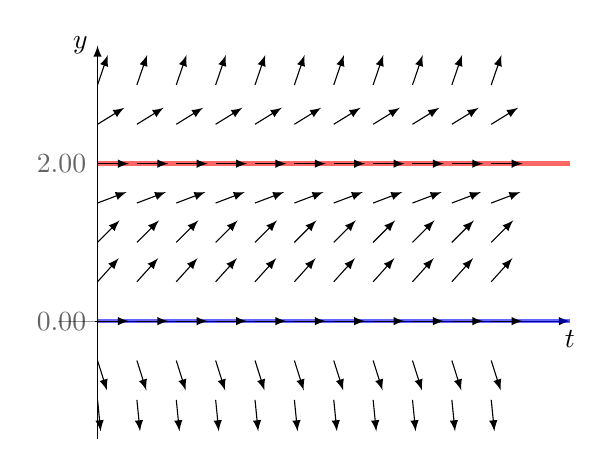
\begin{tikzpicture}
  \draw[-latex] (-0.50, 0)--(6.00, 0) node[below] {$t$};\draw[-latex] (0, -1.50)--(0, 3.50) node[left] {$y$}; \draw[ultra thick, opacity=0.6, blue] (6.00, 0.00)--(0.00, 0.00) node[left, black, fill=white] {$0.00$}; \draw[ultra thick, opacity=0.6, red] (6.00, 2.00)--(0.00, 2.00) node[left, black, fill=white] {$2.00$};\draw[-latex] (0.00, -1.00) -- (0.04 , -1.40);\draw[-latex] (0.00, -0.50) -- (0.12 , -0.88);\draw[-latex] (0.00, 0.00) -- (0.40 , 0.00);\draw[-latex] (0.00, 0.50) -- (0.27 , 0.80);\draw[-latex] (0.00, 1.00) -- (0.28 , 1.28);\draw[-latex] (0.00, 1.50) -- (0.37 , 1.64);\draw[-latex] (0.00, 2.00) -- (0.40 , 2.00);\draw[-latex] (0.00, 2.50) -- (0.34 , 2.71);\draw[-latex] (0.00, 3.00) -- (0.13 , 3.38);\draw[-latex] (0.50, -1.00) -- (0.54 , -1.40);\draw[-latex] (0.50, -0.50) -- (0.62 , -0.88);\draw[-latex] (0.50, 0.00) -- (0.90 , 0.00);\draw[-latex] (0.50, 0.50) -- (0.77 , 0.80);\draw[-latex] (0.50, 1.00) -- (0.78 , 1.28);\draw[-latex] (0.50, 1.50) -- (0.87 , 1.64);\draw[-latex] (0.50, 2.00) -- (0.90 , 2.00);\draw[-latex] (0.50, 2.50) -- (0.84 , 2.71);\draw[-latex] (0.50, 3.00) -- (0.63 , 3.38);\draw[-latex] (1.00, -1.00) -- (1.04 , -1.40);\draw[-latex] (1.00, -0.50) -- (1.12 , -0.88);\draw[-latex] (1.00, 0.00) -- (1.40 , 0.00);\draw[-latex] (1.00, 0.50) -- (1.27 , 0.80);\draw[-latex] (1.00, 1.00) -- (1.28 , 1.28);\draw[-latex] (1.00, 1.50) -- (1.37 , 1.64);\draw[-latex] (1.00, 2.00) -- (1.40 , 2.00);\draw[-latex] (1.00, 2.50) -- (1.34 , 2.71);\draw[-latex] (1.00, 3.00) -- (1.13 , 3.38);\draw[-latex] (1.50, -1.00) -- (1.54 , -1.40);\draw[-latex] (1.50, -0.50) -- (1.62 , -0.88);\draw[-latex] (1.50, 0.00) -- (1.90 , 0.00);\draw[-latex] (1.50, 0.50) -- (1.77 , 0.80);\draw[-latex] (1.50, 1.00) -- (1.78 , 1.28);\draw[-latex] (1.50, 1.50) -- (1.87 , 1.64);\draw[-latex] (1.50, 2.00) -- (1.90 , 2.00);\draw[-latex] (1.50, 2.50) -- (1.84 , 2.71);\draw[-latex] (1.50, 3.00) -- (1.63 , 3.38);\draw[-latex] (2.00, -1.00) -- (2.04 , -1.40);\draw[-latex] (2.00, -0.50) -- (2.12 , -0.88);\draw[-latex] (2.00, 0.00) -- (2.40 , 0.00);\draw[-latex] (2.00, 0.50) -- (2.27 , 0.80);\draw[-latex] (2.00, 1.00) -- (2.28 , 1.28);\draw[-latex] (2.00, 1.50) -- (2.37 , 1.64);\draw[-latex] (2.00, 2.00) -- (2.40 , 2.00);\draw[-latex] (2.00, 2.50) -- (2.34 , 2.71);\draw[-latex] (2.00, 3.00) -- (2.13 , 3.38);\draw[-latex] (2.50, -1.00) -- (2.54 , -1.40);\draw[-latex] (2.50, -0.50) -- (2.62 , -0.88);\draw[-latex] (2.50, 0.00) -- (2.90 , 0.00);\draw[-latex] (2.50, 0.50) -- (2.77 , 0.80);\draw[-latex] (2.50, 1.00) -- (2.78 , 1.28);\draw[-latex] (2.50, 1.50) -- (2.87 , 1.64);\draw[-latex] (2.50, 2.00) -- (2.90 , 2.00);\draw[-latex] (2.50, 2.50) -- (2.84 , 2.71);\draw[-latex] (2.50, 3.00) -- (2.63 , 3.38);\draw[-latex] (3.00, -1.00) -- (3.04 , -1.40);\draw[-latex] (3.00, -0.50) -- (3.12 , -0.88);\draw[-latex] (3.00, 0.00) -- (3.40 , 0.00);\draw[-latex] (3.00, 0.50) -- (3.27 , 0.80);\draw[-latex] (3.00, 1.00) -- (3.28 , 1.28);\draw[-latex] (3.00, 1.50) -- (3.37 , 1.64);\draw[-latex] (3.00, 2.00) -- (3.40 , 2.00);\draw[-latex] (3.00, 2.50) -- (3.34 , 2.71);\draw[-latex] (3.00, 3.00) -- (3.13 , 3.38);\draw[-latex] (3.50, -1.00) -- (3.54 , -1.40);\draw[-latex] (3.50, -0.50) -- (3.62 , -0.88);\draw[-latex] (3.50, 0.00) -- (3.90 , 0.00);\draw[-latex] (3.50, 0.50) -- (3.77 , 0.80);\draw[-latex] (3.50, 1.00) -- (3.78 , 1.28);\draw[-latex] (3.50, 1.50) -- (3.87 , 1.64);\draw[-latex] (3.50, 2.00) -- (3.90 , 2.00);\draw[-latex] (3.50, 2.50) -- (3.84 , 2.71);\draw[-latex] (3.50, 3.00) -- (3.63 , 3.38);\draw[-latex] (4.00, -1.00) -- (4.04 , -1.40);\draw[-latex] (4.00, -0.50) -- (4.12 , -0.88);\draw[-latex] (4.00, 0.00) -- (4.40 , 0.00);\draw[-latex] (4.00, 0.50) -- (4.27 , 0.80);\draw[-latex] (4.00, 1.00) -- (4.28 , 1.28);\draw[-latex] (4.00, 1.50) -- (4.37 , 1.64);\draw[-latex] (4.00, 2.00) -- (4.40 , 2.00);\draw[-latex] (4.00, 2.50) -- (4.34 , 2.71);\draw[-latex] (4.00, 3.00) -- (4.13 , 3.38);\draw[-latex] (4.50, -1.00) -- (4.54 , -1.40);\draw[-latex] (4.50, -0.50) -- (4.62 , -0.88);\draw[-latex] (4.50, 0.00) -- (4.90 , 0.00);\draw[-latex] (4.50, 0.50) -- (4.77 , 0.80);\draw[-latex] (4.50, 1.00) -- (4.78 , 1.28);\draw[-latex] (4.50, 1.50) -- (4.87 , 1.64);\draw[-latex] (4.50, 2.00) -- (4.90 , 2.00);\draw[-latex] (4.50, 2.50) -- (4.84 , 2.71);\draw[-latex] (4.50, 3.00) -- (4.63 , 3.38);\draw[-latex] (5.00, -1.00) -- (5.04 , -1.40);\draw[-latex] (5.00, -0.50) -- (5.12 , -0.88);\draw[-latex] (5.00, 0.00) -- (5.40 , 0.00);\draw[-latex] (5.00, 0.50) -- (5.27 , 0.80);\draw[-latex] (5.00, 1.00) -- (5.28 , 1.28);\draw[-latex] (5.00, 1.50) -- (5.37 , 1.64);\draw[-latex] (5.00, 2.00) -- (5.40 , 2.00);\draw[-latex] (5.00, 2.50) -- (5.34 , 2.71);\draw[-latex] (5.00, 3.00) -- (5.13 , 3.38);
\end{tikzpicture}
\end{figure}

Como ilustra o campo de direções acima, o comportamento das soluções quando \(t \rightarrow \infty\) depende do valor inicial de \(y\) em \(t = 0\). De fato, seja a condição inicial \(y_0 = y(t=0)\). Então

\begin{itemize}
    \item Para $y_0 < 0$, as soluções afastam-se da solução de equilíbrio $y =0$ e tendem a $-\infty$.
    \item Para $y_0 > 2$, as soluções afastam-se da solução de equilíbrio $y =2$ e tendem a $+\infty$.
    \item Para $0 < y_0 < 2$, as soluções afastam-se da solução de equilíbrio $y =0$ e tendem à solução $y = 2$.
\end{itemize}
\fimSol

\begin{enumerate}
  \setcounter{enumi}{20}
  \item Um pequeno lago contém, inicialmente, 1.000.000 galões (aproximadamene 1.550.000 litros) de água e uma quantidade deswconhecida de um produto químico indesejável. O lago recebe água contendo 0,01 grama dessa subtância por gação a uma taxa de 300 galões por hora. A mistura sai à mesma taxa, de modo que a quantidade de água no lago permanece constante. Suponha que o produto esteja distribuído uniformemente no lago.
  \begin{enumerate}[label=(\alph*)]
    \item Escreva uma equação diferencial para a quantidade de produto químico no lago em um instante qualquer.\\
    %%
    \iniSol
    Seja $Q(t)$ a quantidade da substância presente no lago no instante de tempo $t$. 
    \fimSol
    \item Qual a quantidade de produto químico que estará no lago após um período muito longo de tempo? Essa quantidade-limite depende da quantidade presente inicialmente?
  \end{enumerate}
\end{enumerate}

\begin{enumerate}[resume]
  \item Uma gota de chuva esférica evapora a uma taxa proporcional à sua área de superfície. Escreva uma eequação diferencial para o volume de uma gota de chuva em função do tempo.
\end{enumerate}

\iniSol

Se a gota evapora a uma taxa proporcional à sua área superficial, temos:
\[
  \dfrac{dV}{dt} = - c S
  \]
em que \(V\) é o volume da gota, \(S\) é a área superficial e \(c\) é uma constante positiva que depende das condições do problema. O sinal negativo indica que a gota perde volume enquanto evapora.

Sabendo que a gota possui formato esférico, temos:
\begin{align*}
    \begin{cases}
      V = \dfrac{4}{3} \pi r^3\\
      S = 4 \pi r^2
    \end{cases}
    &\Rightarrow 
    \dfrac{V^2}{S^3} = \dfrac{\left(\dfrac{4}{3}\pi r^3\right)^2}{\left(4\pi r^2\right)^3} = \dfrac{\dfrac{16}{9} \pi^2 r^6}{64 \pi^3 r^6} = \dfrac{1}{36 \pi} = \text{constante}\\
    &\Rightarrow S^3 = 36\pi V^2\\
    &\Rightarrow S = \sqrt{36\pi} V^{2/3}
  \end{align*}
Substituindo na equação diferencial acima, tem-se:
\[
  \dfrac{dV}{dt} = -k V^{2/3}
  \]
em que \(k = \sqrt{36 \pi} \cdot c\).
\fimSol

\begin{enumerate}[resume]
  \item A lei do resfriamento de Newton dz que a temperatura de um objeto varia a uma taxa proporcional à diferença entre a temperatura do objeto e a temperatura do meio em que está inserido ( a temperatura do ambiente, na maior parte dos casos). Suponha que a temperatura ambienete é $70^\circ$F (cerca de $21^\circ$C) e que a taxa é de 0,05 por minuto. Escreva uma equação diferencial para a temperatura do objeto em qualquer instante $t$
\end{enumerate}

\iniSol

Seja \(T(t)\) a temperatura do objeto no instante \(t\). Definimos ainda \(T_a = 70^\circ\)F a temperatura do ambiente e \(k = 0,05\) a taxa de proporcionalidade. Seja ainda \(\dfrac{dT}{dt}\) a taxa de variação da temperatura do objeto. Façamos algumas considerações:

\begin{itemize}
    \item Se $T(t) = T_a$ (ou $T - T_a = 0$), não há troca de calor entre o objeto e o ambiente e a temperatura do objeto não sofre variação. Nesse caso, $\dfrac{dT}{dt} = 0$.
    \item Se $T(t) > T_a$ (ou $T - T_a > 0$), o objeto perde calor e sua temperatura tende a diminuir. Nesse caso, $\dfrac{dT}{dt} < 0$.
    \item Se $T < T_a$ (ou $T - T_a < 0$) o objeto recebe calor do ambiente e sua temperatura tende a aumentar. Nesse caso, $\dfrac{dT}{dt} > 0$.
  \end{itemize}

Assim, observamos que o sinal da taxa de variação \(\dfrac{dT}{dt}\) é sempre contrário ao sinal da diferença \(T - T_a\). Portanto, a equação diferencial que descreve o fenômeno é:
\[
  \dfrac{dT}{dt} = -k (T - T_a)
  \]
\fimSol

\begin{enumerate}
  \setcounter{enumi}{24}
  \item Para pequenos objetos, caino devagar, a hipótese feita no texto sobre a resistência do ar ser proporcional à velocidade é boa. Para objetos maiores, caindo mais rapidamente, é mais preciso supor que a resistência do ar é proporcional ao quadrado da velocidade.
  \begin{enumerate}[leftmargin=*, label=(\alph*)]
    \item Escreva uma equação diferencial para a velocidade de um objeto em queda de massa $m$ se a resistência do ar é proporcional ao quadrado da velocidade.\\
    %%
    \iniSol
      O diagrama abaixo mostra as forças envolvidas durante o movimento de queda:
      \begin{figure}[H]
        \centering
        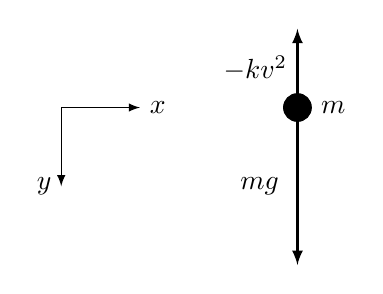
\begin{tikzpicture}
          \filldraw (0,0) circle (5pt) node[right, xshift=5pt] {$m$};
          \draw[thick, -latex] (0,0) -- (0, -2) node[midway, left, xshift=-3pt] {$mg$};
          \draw[thick, -latex] (0,0) -- (0, 1) node[midway, left] {$-kv^2$};
          \draw[latex-latex] (-2, 0) node[right] {$x$} -- ++(-1, 0) -- ++(0, -1) node[left] {$y$};
        \end{tikzpicture}
      \end{figure}
      Aplicando a Segunda Lei de Newton, obtemos a seguinte equação diferencial para a velocidade $v$ durante a queda:
      $$
      m \dfrac{dv}{dt} = mg - kv^2 \Rightarrow \dfrac{dv}{dt} = g - \dfrac{k}{m}v^2
      $$
    \fimSol
    \item Determine a velocidade-limite após um longo período de tempo.\\
    %%
    \iniSol
      Durante a queda, a velocidade do objeto tende a aumentar, devido à ação da aceleração da gravidade $g$. Por sua vez, a resistência do ar $-kv^2$ também cresce em módulo, mas somente até atingir o equilíbrio com a força peso $mg$. Assim, a velocidade-limite será dada por:
      \begin{align*}
        \dfrac{dv}{dt} = 0 &\Rightarrow g - \dfrac{k}{m}v_{lim}^2 = 0\\
        &\Rightarrow v_{lim}^2 = \dfrac{mg}{k}\\
        &\Rightarrow v_{lim} = \sqrt{\dfrac{mg}{k}}
      \end{align*}
    \fimSol
  \end{enumerate}
\end{enumerate}

\end{document}
